%! TEX program = xelatex

\documentclass{report}
\usepackage[UTF8, heading=true]{ctex}
\usepackage{fancyhdr}
\usepackage{tocloft}
\usepackage[margin=1in]{geometry}
\usepackage{metalogo}                   % \XeLaTeX
\usepackage{float}                      % figure H flag
\usepackage{microtype}                  % break long words
\usepackage[bottom]{footmisc}           % force footnote stay bottom
\usepackage{listings}                   % code
\usepackage{xparse}                     % newcommand multiple optional arguments
\usepackage[hidelinks]{hyperref}
\usepackage{tabularx}
\usepackage{enumitem}
\usepackage{algorithm}                  % algorithm pseudo code
\usepackage[noend]{algpseudocode}
\usepackage{caption}

\usepackage{amsmath}                    % advanced math support
\usepackage{lmodern}                    % allow font to scale

% make chapter stay in the same page
%\makeatletter
%\renewcommand\chapter{\thispagestyle{plain}%
%\global\@topnum\z@
%\@afterindentfalse
%\secdef\@chapter\@schapter}
%\makeatother

% settings %%%%%%%%%%%%%%%%%%
%%%%%%%%%%%%%%%%%%%%%%%%%%%%%

\ctexset{
    chapter = {
        format += \flushleft,
        %beforeskip = 20pt,
        number = \chinese{chapter},
        name = {实验},
    },
    section = {
        format += \flushleft,
    },
    appendix = {
        number = \Alph{chapter},
        name = {附录},
    },
}

\pagestyle{fancy}
\graphicspath{{./res/}}
\hypersetup{bookmarksopenlevel=2}

% defines %%%%%%%%%%%%%%%%%%%
%%%%%%%%%%%%%%%%%%%%%%%%%%%%%
\NewDocumentCommand{\inputCode}{ O{c} m }{
    {
        \setmainfont{FiraCode Nerd Font}[
            ItalicFont  = FiraCode Nerd Font
        ]
        \lstinputlisting[
            basicstyle=\codeF,
            language=#1,
            tabsize=4,
            showstringspaces=false,
            breaklines=true,
            frame=shadowbox,
            framexleftmargin=10mm,
            rulesepcolor=\color{black},
            basicstyle=\small,
            numbers=left,
            xleftmargin=3em,
        ]{#2}
    }
}
\NewDocumentEnvironment{simpleAlgorithm}{m}
{
\captionof{algorithm}{#1}
\hrule
\begin{algorithmic}[1]
} {
\end{algorithmic}
\hrule \vspace{1em}
}

% report content %%%%%%%%%%%%
%%%%%%%%%%%%%%%%%%%%%%%%%%%%%
\begin{document}

\begin{titlepage}
    \addtolength{\topmargin}{1cm}
    \centering
    
\includegraphics[width=0.6\textwidth]{hust.jpg}\par
    \vspace{0.5cm}
    {\Huge \heiti 算法设计与分析实验报告}\par
    \vspace{10cm}
    {
        \large
        \begin{tabular}{r m{8em}}
            \makebox[6em][s]{学生姓名}:& 胡思勖 \\ \cline{2-2}
            \makebox[6em][s]{学号}:& U201514898\\ \cline{2-2}
            \makebox[6em][s]{专业}:& 计算机科学与技术\\ \cline{2-2}
            \makebox[6em][s]{班级}:& 计卓1501\\ \cline{2-2}
            \makebox[6em][s]{指导教师}:& 王多强\\ \cline{2-2}
        \end{tabular}
    }
    \vfill
    2017年12月25日
\end{titlepage}

\setcounter{tocdepth}{1}
\tableofcontents
\newpage

% Chapter One %%%%%%%%%%%%%%%
%%%%%%%%%%%%%%%%%%%%%%%%%%%%%
\chapter{最近点对问题}
\label{cha:zui_jin_dian_dui_wen_ti_}

\section{题目描述}
\label{sec:ti_mu_miao_shu_1}

给出平面上的一些点的坐标,求出距离最近的两个点的坐标。如果有多对距离相同的点,依次输出这些点的坐标。\par
测试文件格式:\par
\begin{itemize}
    \item 输入文件:in.dat
        \begin{itemize}
            \item 格式:第一行为一个整数,表示测试用例的组数,其后跟相应组数的测试用例
            \item 每组测试用例包括:
                \begin{itemize}
                    \item 首行:一个整数,表示本组测试用例包含的点数,其后跟相应点数的行
                    \item 其后:每行两个整数,表示该点的 x、y 坐标
                \end{itemize}
        \end{itemize}
    \item 输出文件:out.dat
        \begin{itemize}
    \item 格式:每行输出一个测试用例的答案,即本组测试用例中相距最近的两个点,用点的坐标表示:四个整数。前两个整数表示第一个点,后两个整数表示第二个点。若有多对相距最近的点,依次罗列。
        \end{itemize}
\end{itemize}

\section{算法设计}
\label{sec:suan_fa_she_ji_1}
最符合直觉的方法为朴素算法,即枚举空间中所有可能的点对,并分别计算这些点对之间的距离,最小的那个距离即为答案。即$\min\{distance(p_i, p_j)\mid i,j\in[1, n]\}$,其中$p_i$、$p_j$是输入中的点,$n$是输入的规模,需要对于$(i, j)$进行枚举,时间复杂度为$O(N^{2})$。\par

然而朴素算法的时间复杂度过高,使用分治法将问题分解成更小的问题,并当问题的规模足够小时直接求解可以降低整体运算的时间复杂度。首先将输入的点按照其横坐标排序,然后取这些横坐标的中位数讲平面划分为左右两部分,这样使近似一半的点进入左半部分,另一半的点进入右半部分,这样将原来的问题划分为两个子问题:以左半部分点集P为输入的子问题和以右半部分点集Q为输入的子问题。对于原问题而言,其解只有三种情况:
\begin{itemize}
    \item 最小距离点对的两个点均在P中。
    \item 最小距离点对的两个点均在Q中。
    \item 最小距离点对的两个点一个在P中,另一个在Q中。
\end{itemize}
对于第一种和第二种情况需要常数时间进行合并,但是若出现第三情况,对于左半部分中的任意一点右半部分中最多有n/2个点需要进行距离的计算,此时合并步骤的耗时为$O(N^{2})$,整个算法的计算时间也为$O(N^{2})$,与朴素算法相同。可以看到,在整个算法中是由于合并阶段的第三种情况导致的计算时间复杂度过高,因此要对这一部分进行限制。\par

假设P中的最近点对和Q中的最近点对已经求得,分别为${p_1, p_2}$和${q_1, q_2}$,并令$\theta$为这两个点对距离中较小的那一个,那么若平面上最小距离点对属于第三种情况(一个点在P中,另一个在Q中),则在这一点对${p_3, q_3}$中,$p_3$与用于划分的中点$m$的横坐标距离不超过$\theta$,否则$p_3$与$q_3$之间的距离将会超过$\theta$,从而与这是最小距离点对矛盾。同理,可以将$q_3$的横坐标限制在$[x_m, x_m+\theta]$范围内,这样就将第三种情况中需要计算的点对限制在了$x\in [x_m-\theta, x_m+\theta]$这样一个带状区域内。又由于$p_3$与$q_3$之间的距离小于$\theta$,因此从纵坐标来看,对于带状区域中的每一个点k只需要计算$y\in [y_k-\theta, y_k+\theta]$这一区域的点。从而对于带状区域中的每一个点,只需要检查$\theta \times 2\theta$的一个矩形中的点即可,如图\ref{fig:example1}所示,对于带状区域左半部分中的点k,在右半部分找到对应的高为$2\theta$,宽为$\theta$的矩形并依次计算k与这一矩形中的点的距离即可。
\begin{figure}[ht]
    \centering
    \begin{minipage}{.45\textwidth}
        \centering
        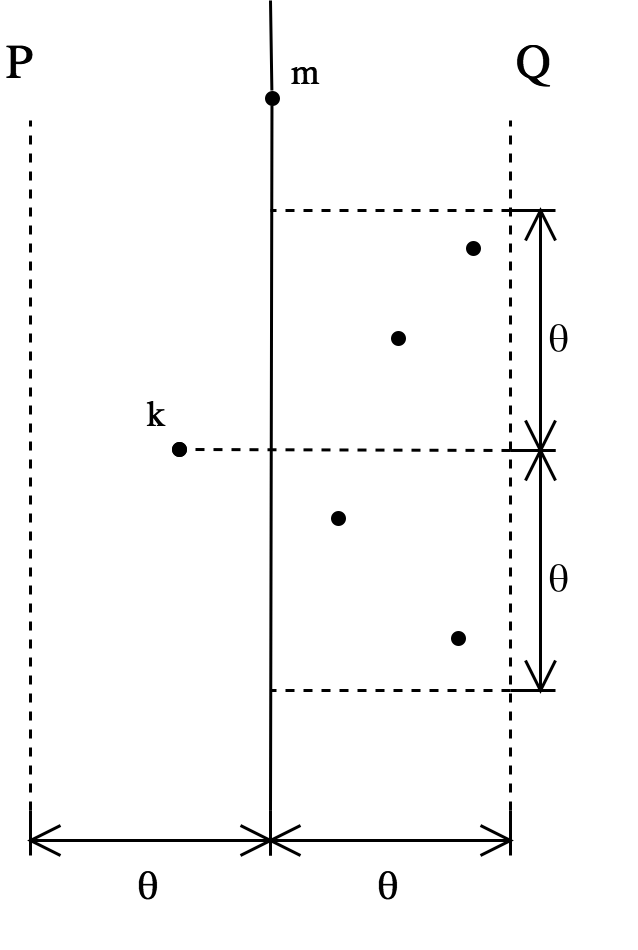
\includegraphics[width=0.6\linewidth]{example1.png}
        \caption{包含点$q_3$的矩形}
        \label{fig:example1}
    \end{minipage}
    \begin{minipage}{.45\textwidth}
        \centering
        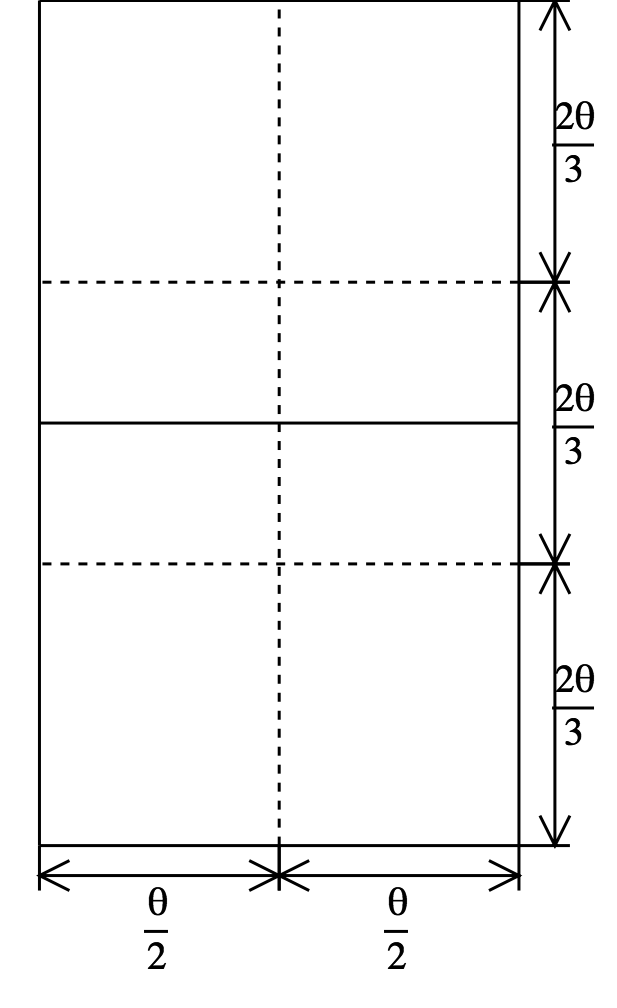
\includegraphics[width=0.5\linewidth]{example2.png}
        \caption{矩形中点的个数}
        \label{fig:example2}
    \end{minipage}
\end{figure}
此外,可以证明这一矩形中的点不超过6个:将点k对应的矩形按照如\ref{fig:example2}所示的方式划分为6个$\frac{\theta}{2}\times\frac{2\theta}{3}$的矩形,由于在右半部分没有两个点之间的距离小于$\theta$因此对于这6个矩形而言每个矩形中至多只有一个点,因为一个矩形中最大的两个点的距离为对角线长,即为$\sqrt{(\frac{\theta}{2})^{2}+(\frac{2\theta}{3})^{2}}\approx0.83\theta<\theta$,因此在这种合并步骤中,对于第三种情况至多只需要检查$6\times n/2=3n$对点,而若这所有点是按照纵坐标进行排序过的,那么只需要$O(n)$的时间就可以完成合并操作,此时最终的时间复杂度为$O(n\log{n})$。

从上述过程即可构建程序的伪代码:\par
\begin{simpleAlgorithm}{寻找最近点对算法}
    \Procedure{FindNearestDotPairs}{$S$}
    \State 将$S$按照横坐标为中位数的点m近似划分为两等分$P,Q$
    \State $(A_1, d_1) \gets $ \Call{FindNearestDotPairs}{$P$}
    \State $(A_2, d_2) \gets $ \Call{FindNearestDotPairs}{$Q$}
    \State $\theta \gets \min\{d_1, d_2\}, d \gets \min\{d_1, d_2\}, A \gets \min\{A_1, A_2\}$
    \For{$k$ in left half of $x\in[x_m-\theta, x_m+\theta]$}
        \For{$j$ in $x\in[x_m, x_m+\theta], y\in[y_k-\theta, y_k+\theta]$}
        \If{$distance(j, k) < d$}
            \State $d \gets distance(j, k)$
            \State $A \gets \{j, k\}$
        \ElsIf{$distance(j, k) = d$}
            \State $A \gets A \bigcup \{j, k\}$
        \EndIf
        \EndFor
    \EndFor
    \State \Return (A, d)
    \EndProcedure
\end{simpleAlgorithm}

将此程序按照递归部分划分,分为主函数和fingNearestDotPairts函数这两个过程,程序的流程图如\ref{fig:flowchart1}所示,其中主函数负责对于输入点集的稳定排序以及调用findNearestDotPairs过程,findNearestDotPairs则递归调用自身寻找最小点对。
\begin{figure}[ht]
    \centering
    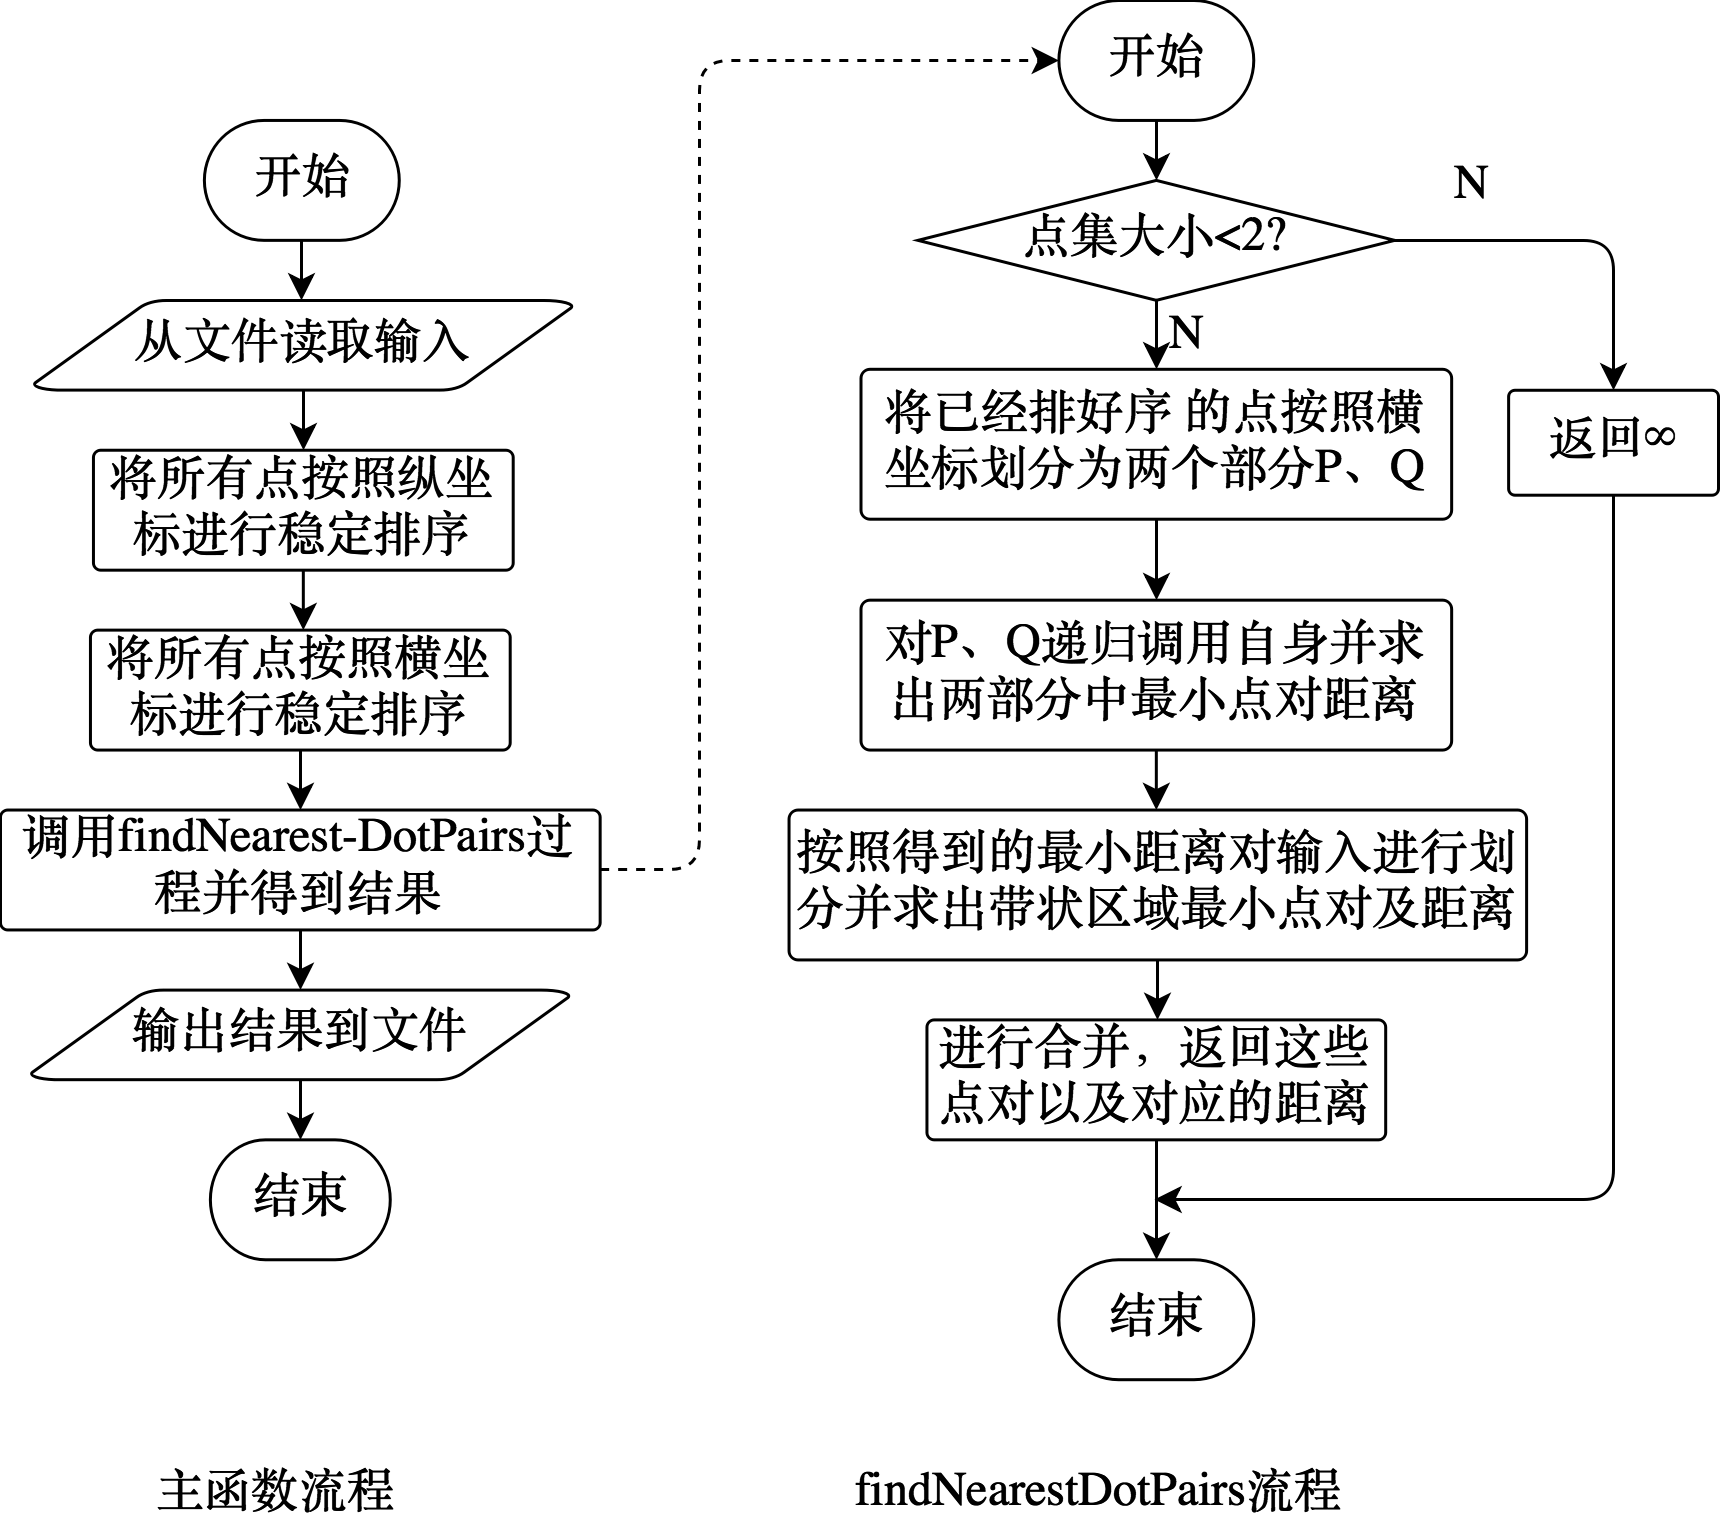
\includegraphics[width=0.7\linewidth]{flowchart1.png}
    \caption{程序流程图}
    \label{fig:flowchart1}
\end{figure}

\section{测试分析}
\label{sec:ce_shi_fen_xi_1}
将源程序编译后进行测试,输入样例为给定的1\_self/in.dat,共有两组输入,第一组输入的点为$(1, 9), (3, 8), (4, 6), (8, 1)$,第二组输入的点为$(10, 8), (23, 98), (18, 32), (78, 43), (76, 25)$。对于第一组结果而言,期望得到的结果为${(1, 9), (3, 8), (3, 8), (4, 6)}$,其最小距离为$\sqrt{5}$;对于第二组数据,期望得到的结果为${(76, 25), (78, 43)}$,最小距离为$2\sqrt{82}$,运行程序的过程以及得到的结果如图\ref{fig:result1}所示,这与预期的结果一致,可以看出这一算法能够成功的计算出所有距离最小的点对。
\begin{figure}[ht]
    \centering
    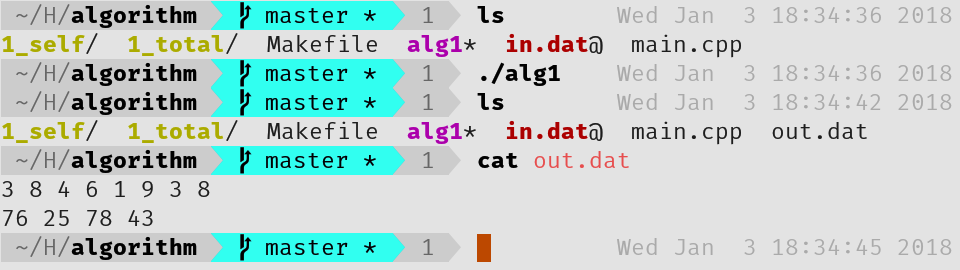
\includegraphics[width=0.8\linewidth]{result1.png}
    \caption{测试结果}
    \label{fig:result1}
\end{figure}

\section{技术总结}
\label{sec:ji_zhu_zong_jie_1}
这一问题是一个典型的使用分治法解决的问题。为了降低这一算法的时间复杂度,我们首先对于算法中最占用时间的部分进行分析,发现是合并操作导致了时间占用最长后,通过已知条件限制合并操作处理的数据量的大小来减少合并时间,其中,证明每一个$\theta \times 2\theta$的矩形中至多只有6个点(即点的稀疏性)是关键的一步,这直接导致了在处理合并操作时时间复杂度从$O(N^2)$降为$O(N)$而使得整个程序的时间复杂度下降。\par

在程序实现时,使用两次稳定排序先后处理纵坐标和横坐标是使得后续处理所用时间较少的关键,这样可以在合并操作时不需要重新对于部分输入的点进行排序,对于两个点分别在左右两边的情况,能够将每次查找的点限制在一个较为连续的内存中,使得在首次遇到超出矩形范围的点时即可跳出循环,进行下一轮比较,从而降低程序的运行时间。\par

% Chapter Two %%%%%%%%%%%%%%%
%%%%%%%%%%%%%%%%%%%%%%%%%%%%%
\chapter{大数乘法}
\label{cha:da_shu_cheng_fa_}

\section{题目描述}
\label{sec:ti_mu_miao_shu_2}

利用分治法设计一个计算两个n位的大整数相乘的算法,要求计算时间低于$O(n^{2})$。\par

大整数(biginteger):位数很多的整数,普通的计算机不能直接处理,如: \par
\begin{centering}
9,834,975,972,130,802,345,791,023,498,570,345\par
\end{centering}
对大整数的算术运算,显然常规程序语言是无法直接表示的。编程实现大整数的加、减、乘运算,需考虑操作数为0、负数、任意位等各种情况。\par

测试文件格式:\par
\begin{itemize}
    \item 输入文件:in.dat
        \begin{itemize}
            \item 格式:第一行为一个整数,表示测试用例的组数,其后跟相应组数的测试用例。每个测试用例一行,包含 3 个整数(长整数数字串),前两个是待测试的操作数,第 3 个整数表示操作类型(1:加法,2:减法,3:乘法)。
        \end{itemize}
    \item 输出文件:out.dat
        \begin{itemize}
    \item 格式:每组测试用例输出一行,最后不要加空行
        \end{itemize}
\end{itemize}

\section{算法设计}
\label{sec:suan_fa_she_ji_2}
对于大数乘法而言,目前已知的方法有模拟法(逐位相乘并进位)、Karatsuba算法、Toom-Cook算法、快速傅里叶变换等。使用模拟方法需要对于其中大数中的每一位都要对另一个大数的所有位进一次乘法和一次加法进行处理(不包括进位),这一算法的时间复杂度为$O(N^{2})$,对于这一问题而言显得过于缓慢。Karatsuba算法为Toom-Cook算法的一个特例,其时间复杂度为$O^{\log{3}/\log{2}}$(将4次乘法减小为3次),而Toom-Cook将9次乘法减小为5次,其时间复杂度为$O^{\log{5}/\log{3}}$,FFT可以以更低的时间复杂度$O(N\cdot\log{(N)\cdot\log{(\log{(N)})}})$进行计算。基于实现容易程度以及乘法精度的考虑,最终采用Karatsuba算法实现两个大数的乘法。\par

Karatsuba基于以下原理:令$x, y$为两个$B$进制的$n$位大整数,对于任意小于$n$的正整数$m$,$x, y$可以写为:
\[
    \begin{cases}
        x = x_1B^{m} + x_0\\
        y = y_1B^{m} + y_0
    \end{cases}
\]
此时,$x\cdot y$可以写为:
\[
    \begin{array}{l l}
        x\cdot y & =(x_1B^m+x_0)(y_1B^m+y_0)\\
                 & =z_2B^{2m}+z_1B^m+z_0
    \end{array}
\]
其中,
\[
    \begin{cases}
        z_0 = x_0y_0\\
        z_1 = x_1y_0 + x_0y_1\\
        z_2 = x_1y_1
    \end{cases}
\]
但是这依然需要计算$4\times N^2/4 = N^2$次乘法。但如果$z_2$和$z_0$已经实现,那么$z_1$可以表示为:
\[
    \begin{array}{l l}
        z_1 & =(x_1+x_0)(y_1+y_0)-x_1y_1-x_0y_0 \\
            & =(x_1+x_0)(y_1+y_0)-z_2-z_0
    \end{array}
\]
于是原本需要4次的乘法在加上依赖关系后变成了3次,通过这一过程对于三次乘法的操作数进行递归调用,再加上其余加减法需要的时间为$O(N)$,可以得到$T(N)=3T(\lceil n/2\rceil)+cn+d$,根据主定理可得时间复杂度为$O(n^{\log_{2}{3}})$。需要注意的是,在计算$(x_1+x_0)(y_1+y_0)$时可能会发生溢出($0\leq \text{\it 结果}\leq2B^m$),对于这种情况需要在计算时加以考虑。\par

对于大数相乘原数中出现负数的情况,首先去掉负号,作为两个无符号整数相乘,最后在结果中根据输入负号的个数决定是否加上负号。此外,在加法和减法的实现中要考虑结果中出现前缀0的情况,需要将这些0去除。其中,核心的无符号大整数算法如下:
\begin{simpleAlgorithm}{无符号大整数相乘算法}
    \Procedure{BigIntMultiply}{$x, y$}
    \If{$x.len < 2$ or $y.len < 2$} \Comment{$a.len$指$a$的长度}
        \State 使用模拟法计算$product \gets x\times y$
        \State \Return $product$
    \EndIf
    \State $m \gets \max\{x.size, y.size\}/2$
    \State 按照$m$将$x, y$分为$x_1, x_0, y_1, y_0$ \Comment{其中$x_0.len=\min\{x.len, m\}, y_0.len=\min\{y.len, m\}$}
    \State $z_0 \gets$ \Call{BigIntMultiply}{$x_0, y_0$}
    \State $z_1 \gets$ \Call{BigIntMultiply}{$(x_1+x_0), (y_1+y_0)$}
    \State $z_2 \gets$ \Call{BigIntMultiply}{$x_1, y_1$}
    \State $product \gets z_2\times 10^{2m} +(z_1-z_2-z_0)\times 10^m +z_0$ \Comment{$z_i\times 10^{j}$使用向字符串尾部添加0实现}
    \State 去除$product$前缀0
    \State \Return $product$
   \EndProcedure
\end{simpleAlgorithm}

在实际实现过程中,主函数获得输入后首先调用BigNumMult函数,BigNumMult函数处理两个大数的符号,然后调用BigNumMultHelper函数对于无符号大整数进行计算。BigNumMultHelper使用的即为上述BitIntMultiply算法。整个算法的流程图如\ref{fig:flowchart2}所示。此外,程序还实现了大整数加法和大整数减法,均使用模拟方法实现,此处不再给出流程图。

\begin{figure}[H]
    \centering
    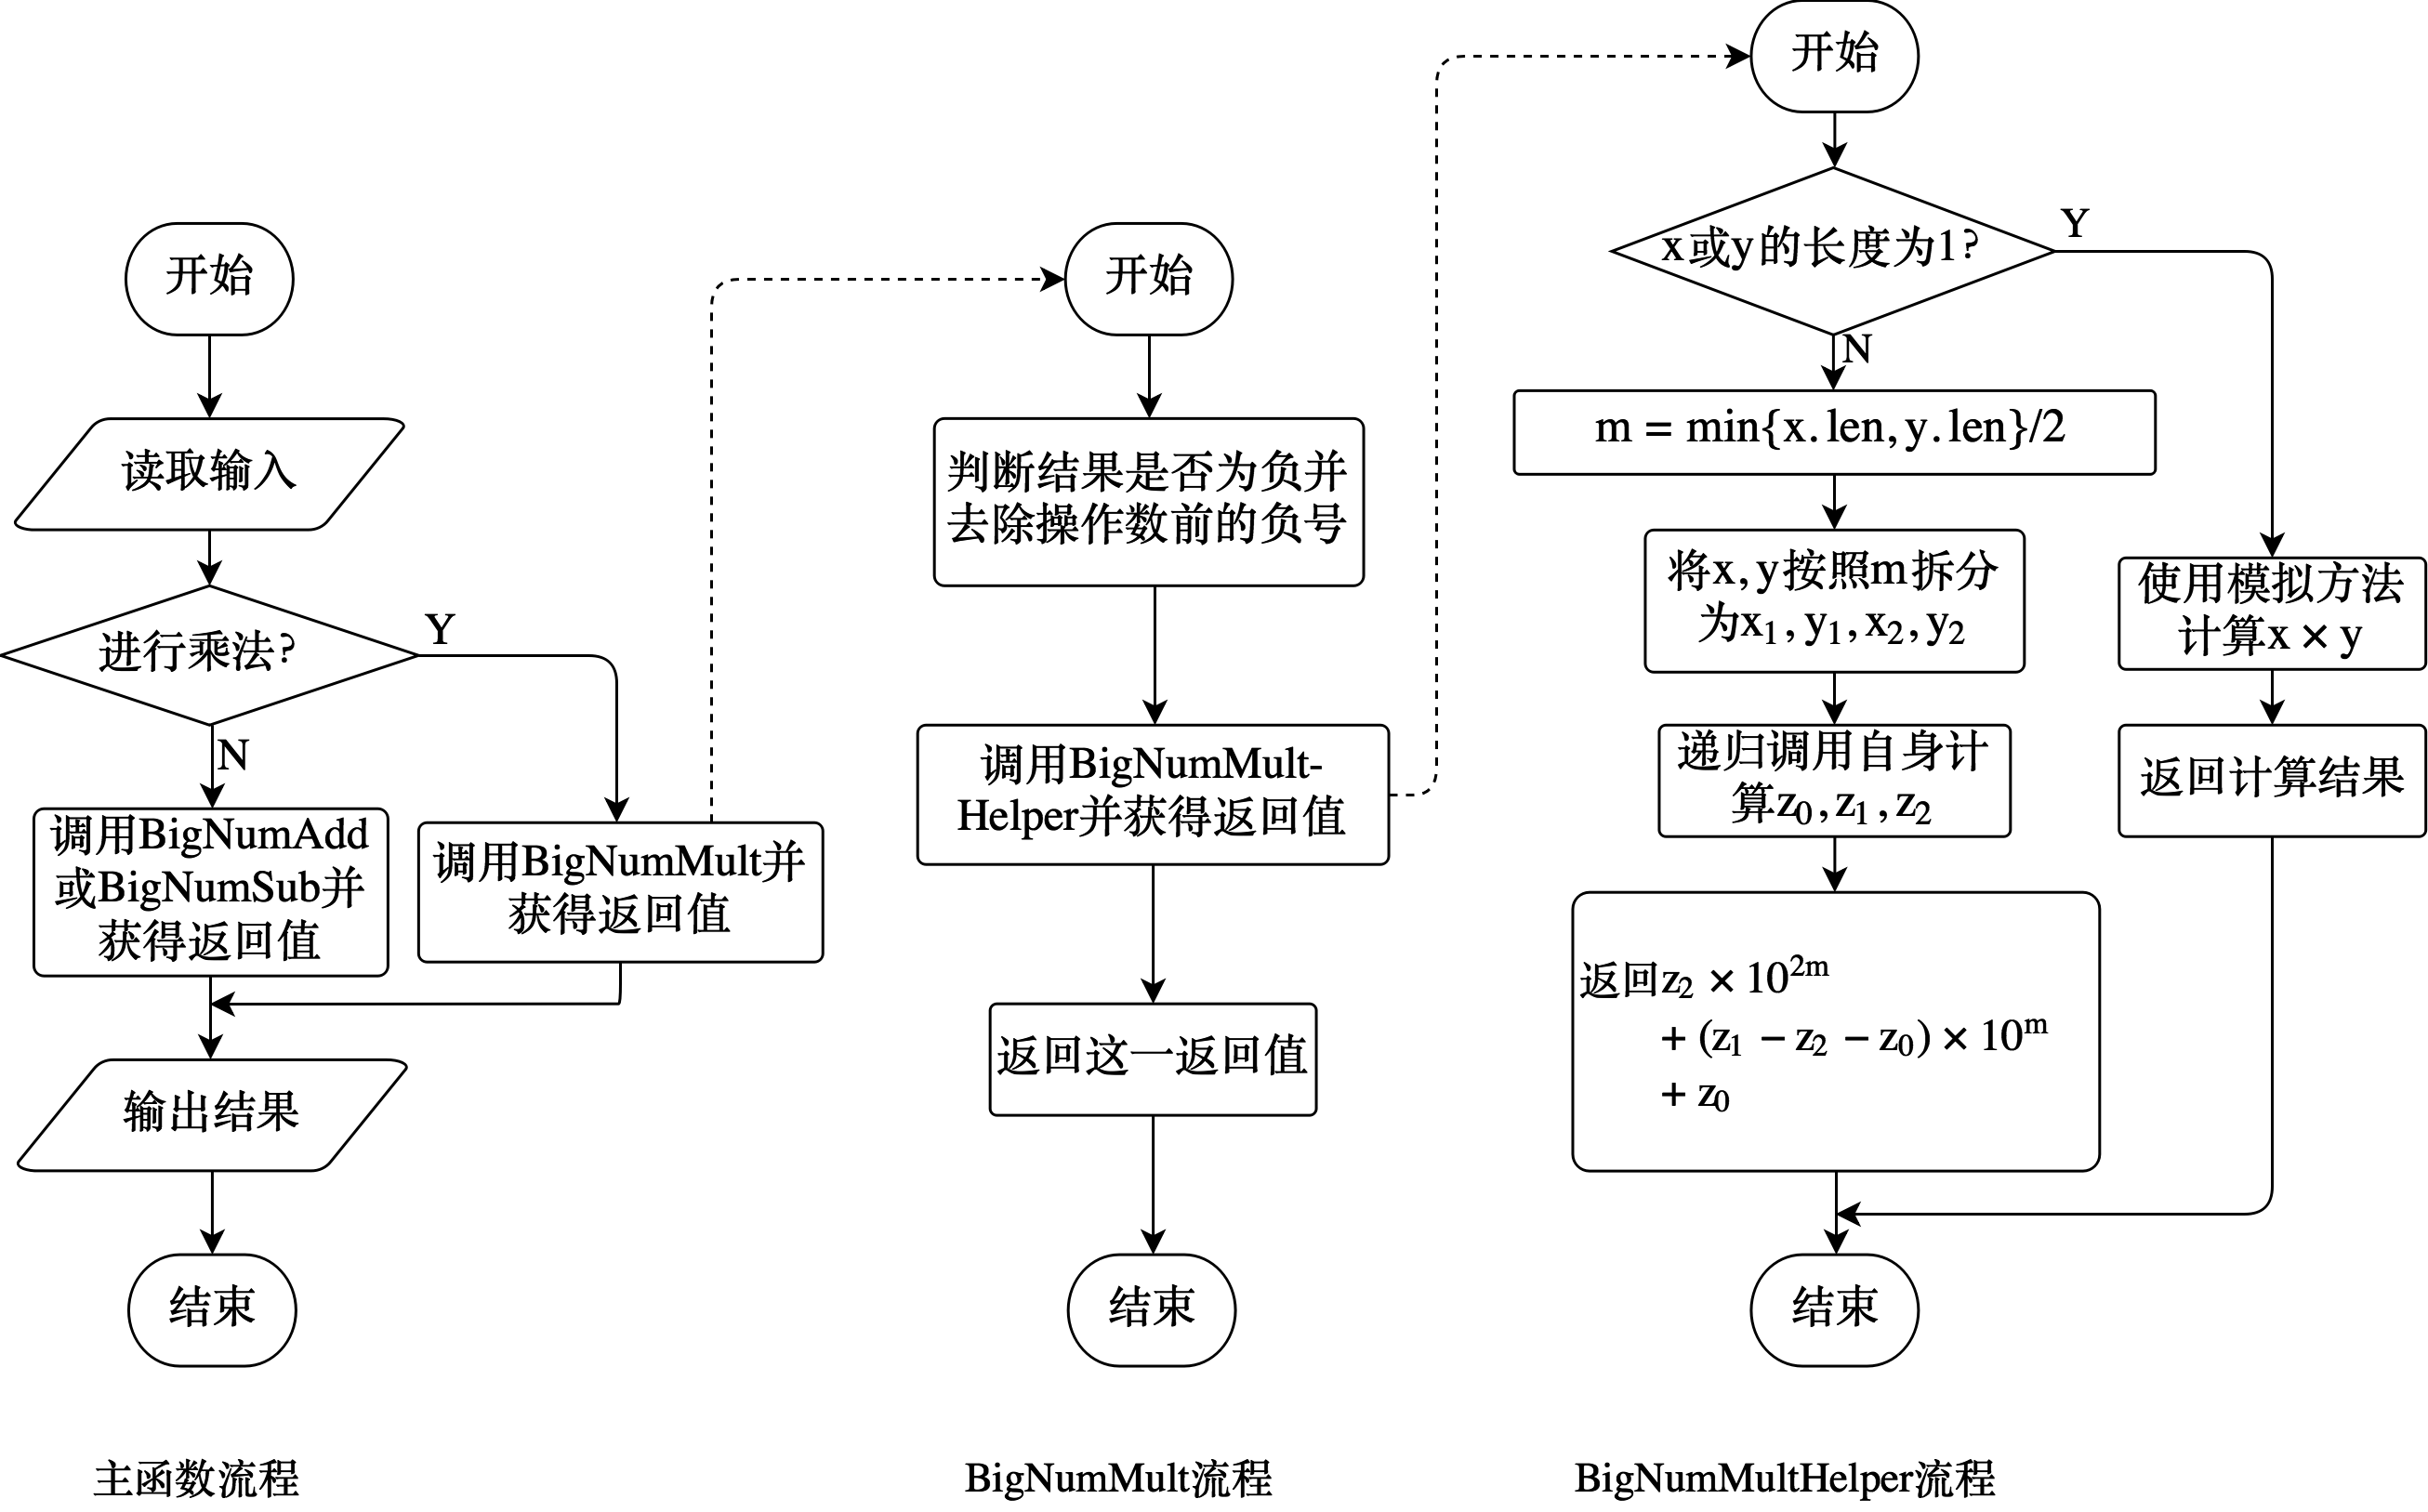
\includegraphics[width=0.9\linewidth]{flowchart2.png}
    \caption{程序大整数乘法部分流程图}
    \label{fig:flowchart2}
\end{figure}

\section{测试分析}
\label{sec:ce_shi_fen_xi_2}
对于程序功能的完整性进行测试,包括对于前缀0的处理,对于负数的处理以及对于大数的处理。输入以及输出如\ref{fig:result2_i}和\ref{fig:result2_o}所示。
\begin{figure}[ht]
    \centering
    \begin{minipage}{.375\textwidth}
        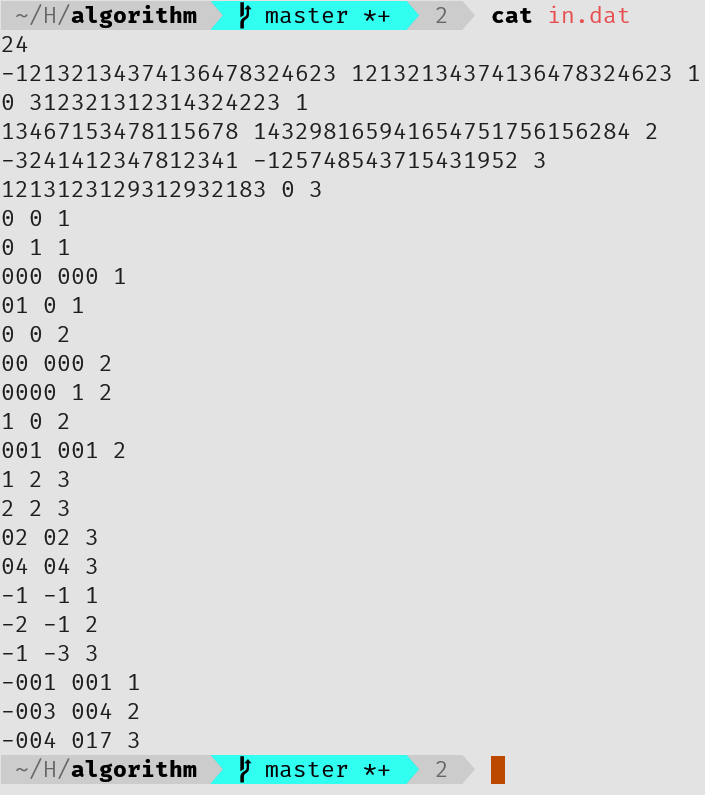
\includegraphics[height=0.3\textheight]{result2_i.png}
        \caption{程序输入}
        \label{fig:result2_i}
    \end{minipage}
    \begin{minipage}{.3\textwidth}
        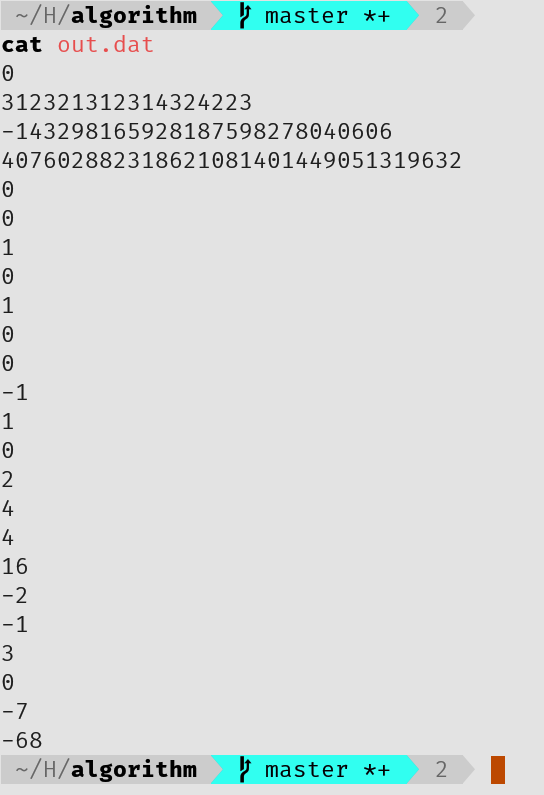
\includegraphics[height=0.3\textheight]{result2_o.png}
        \caption{程序输出}
        \label{fig:result2_o}
    \end{minipage}
\end{figure}
可以看出,对于每一个输入,无论是否有前缀0,输入是否存在负数,程序都能够正确的进行处理,说明程序功能正常。


\section{技术总结}
\label{sec:ji_zhu_zong_jie_2}
在大整数乘法算法中,对于通过数学变换将乘法的次数减少是降低时间复杂度的关键。这一思路在其他算法中也有体现,如Toom-Cook算法以及用于快速矩阵乘法的Strassen算法均是使用这一思想。这种变换值得我们学习并应用在今后的研究过程中。此外,对于负数的处理是值得关注的,在大整数加法和减法的实现中,对于负数的处理应该分情况讨论并调用处理无符号大数加减法的子程序。

% Chapter Three %%%%%%%%%%%%%
%%%%%%%%%%%%%%%%%%%%%%%%%%%%%
\chapter{最优二分查找树}
\label{cha:zui_you_er_fen_cha_zhao_shu_}

\section{题目描述}
\label{sec:ti_mu_miao_shu_3}

\begin{figure}[ht]
    \centering
    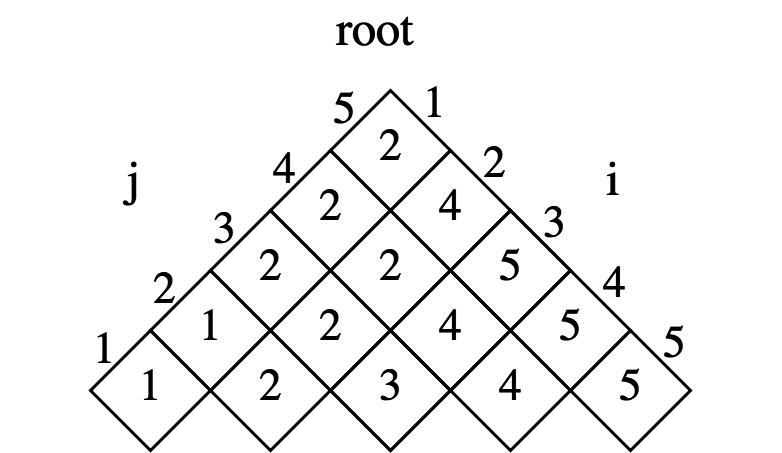
\includegraphics[width=0.35\linewidth]{description3.png}
    \caption{输入表$root$}
    \label{fig:description3}
\end{figure}
设计伪代码CONSTRUCT-OPTIMAL-BST(root),输入为表$root$,输出是最优二叉搜索树的结构。例如,对图\ref{fig:description3}中的$root$表,应输出\par
$k_2$为根\par
$k_1$为$k_2$的左孩子\par
$d_0$为$k_1$的左孩子\par
$d_1$为$k_1$的右孩子\par
$k_5$为$k_2$的右孩子\par
$k_4$为$k_5$的左孩子\par
$k_3$为$k_4$的左孩子\par
$d_2$为$k_3$的左孩子\par
$d_3$为$k_3$的右孩子\par
$d_4$为$k_4$的右孩子\par
$d_5$为$k_5$的右孩子\par

\section{算法设计}
\label{sec:suan_fa_she_ji_3}
由于$root[i,j]$表示的是包含关键字$k_i,...,k_j$子树的根,并且二叉搜索树的子树中的节点都是连续的,因此$root[i,j]$的左子树和又子树的根分别为$root[i, root[i,j]-1]$和$root[root[i,j]+1, j]$,从而可以进行递归找到所有子树的根以及他们与父节点的关系,进而构建整个子树。算法CONSTRUCT-OPTIMAL-BST如下:\par
\begin{simpleAlgorithm}{构建最优子树算法}
    \State Global $k \gets 0$ \Comment{$k$存储伪结点的序号}
    \State Global $result \gets \{\}$ \Comment{$result$采用栈结构}
    \Procedure{Construct-Optimal-Bst}{$root, i, j$}
    \If{$i>j$}
        \State $k \gets k+1$
        \State \Return$nil$
    \EndIf
    \State $child \gets$ \Call{Construct-Optimal-Bst}{$root, root[i,j] + 1, j$}\Comment{找出右孩子}
        \If{$child \neq nil$}
            \State $result$.push (``$child$ 是 $root[i,j]$的右孩子'')
        \Else
            \State $result$.push (``$d_{root.size-k}$ 是 $root[i,j]$的右孩子'')
        \EndIf
        \State $child \gets$ \Call{Construct-Optimal-Bst}{$root, i, root[i,j] - 1$}\Comment{找出左孩子}
        \If{$child \neq nil$}
            \State $result$.push (``$child$ 是 $root[i,j]$的左孩子'')
        \Else
            \State $result$.push (``$d_{root.size-k}$ 是 $root[i,j]$的左孩子'')
        \EndIf
        \State \Return $k_{root[i,j]}$
    \EndProcedure
\end{simpleAlgorithm}

\begin{figure}[ht]
    \centering
    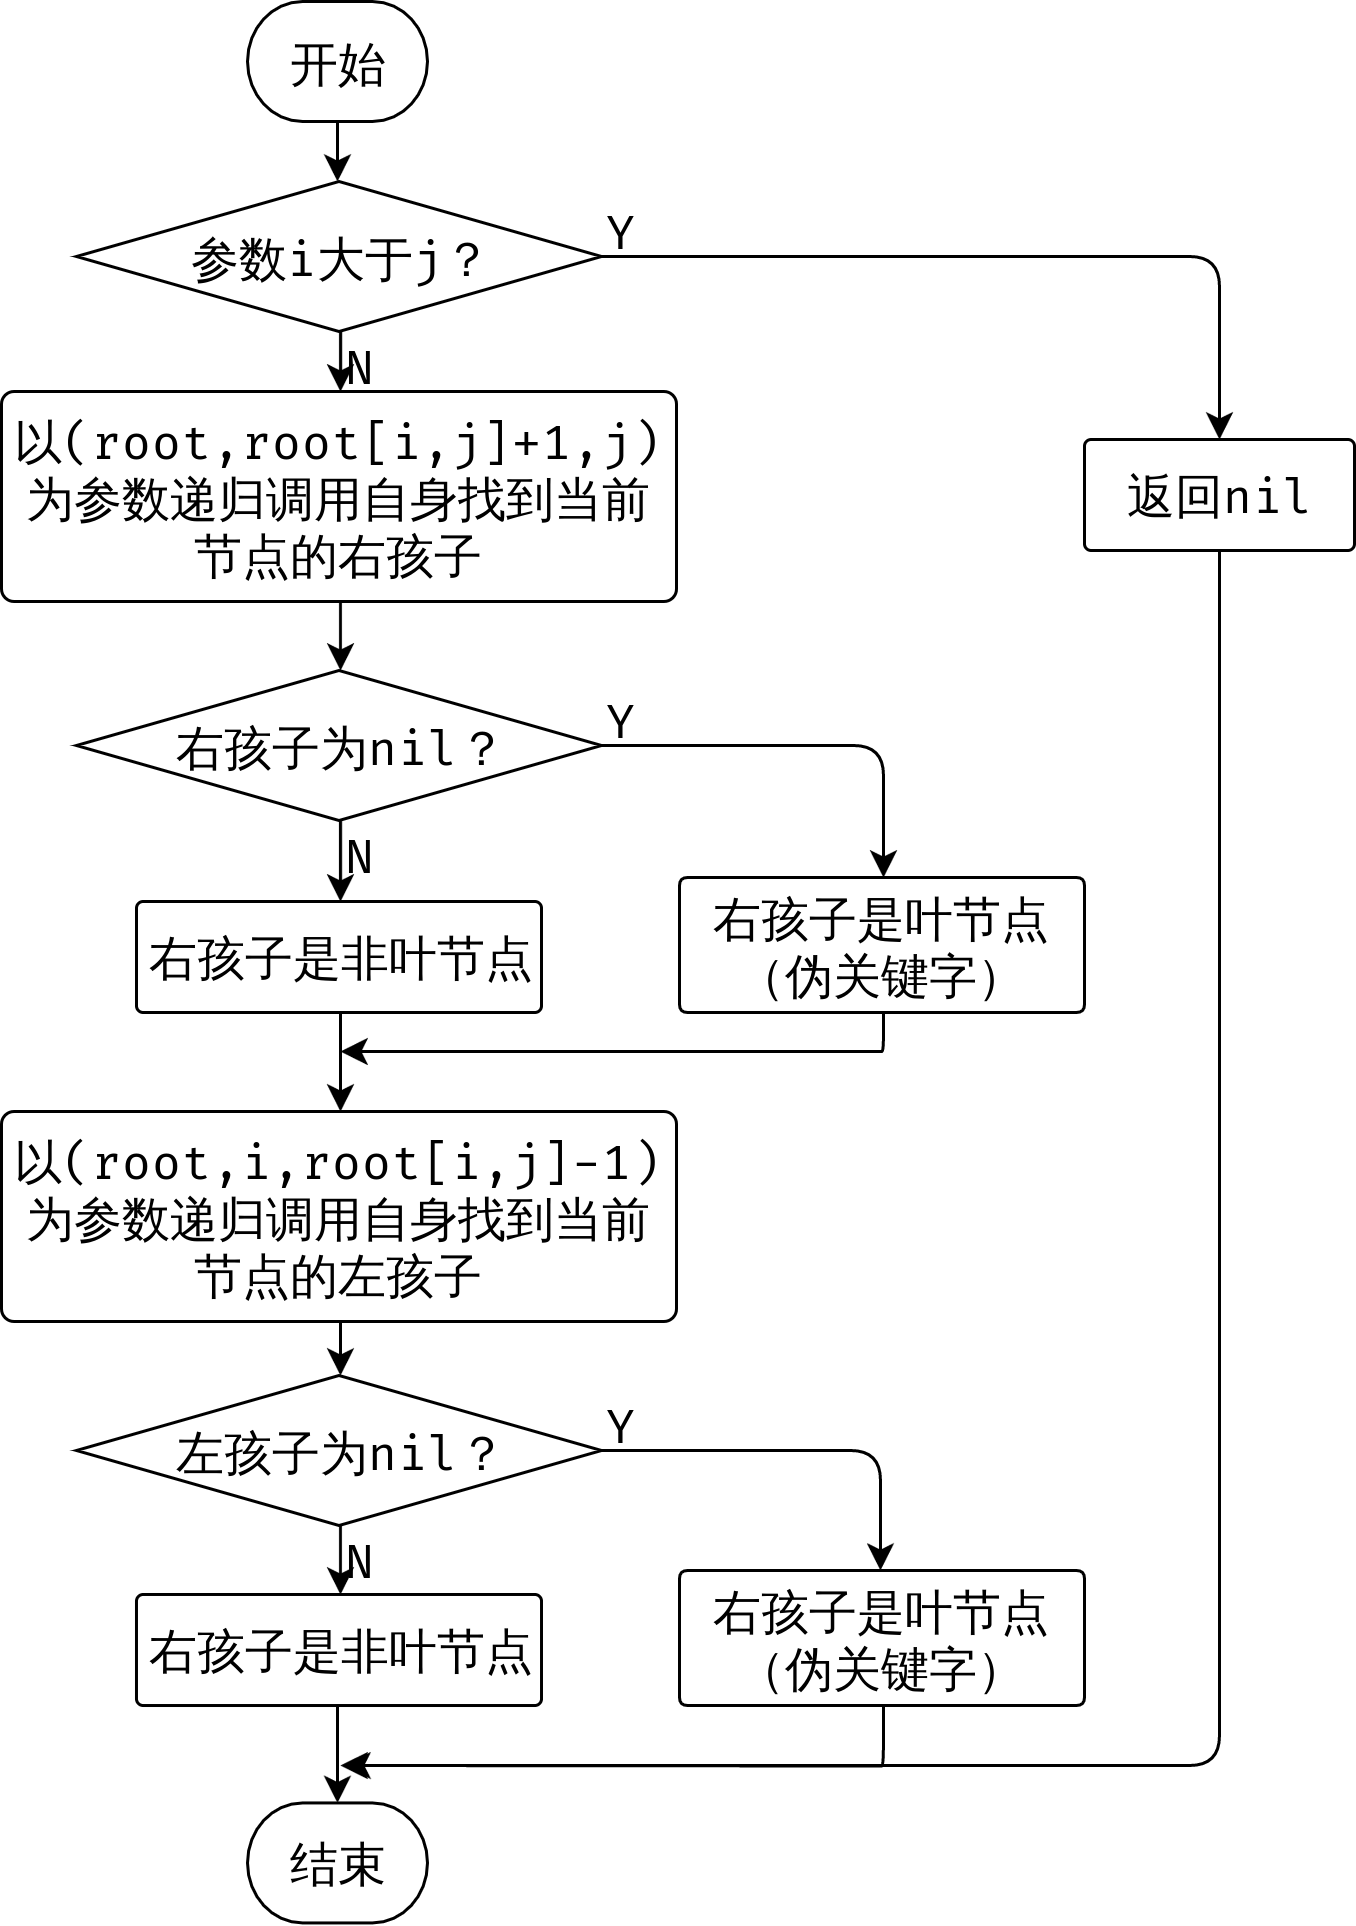
\includegraphics[width=0.4\linewidth]{flowchart3.png}
    \caption{程序流程图}
    \label{fig:flowchart3}
\end{figure}

运行CONSTRUCT-OPTIMAL-BST算法后,从栈$result$中逐个弹出元素并输出即为题目要求的结果。由于在每一层递归中需要在最后返回本节点,因此要按先序遍历的顺序输出,必须按照右孩子-左孩子的顺序遍历并压栈。程序的流程图如图\ref{fig:flowchart3}所示。流程图中给出了构建源二叉树的程序执行框架,没有对于输入输出的细节问题进行详细描绘。\par

在这一递归算法中,每一层递归所需要的参数为$root, i, j$,分别表示整个root表,以及当前节点在root表中的位置$(i, j)$。在每一次递归调用中,若出现$i>j$的情况说明已经到达了叶节点,因为所有的非叶节点在$root$中的的坐标全部满足$i\leq j$,此时返回$nil$以告知调用者已经到达了叶节点。否则递归调用自身,首先确定这一节点的右子树,然后确定这一节点的左子树,最后返回节点自身作为上一层调用的答案。

\section{测试分析}
\label{sec:ce_shi_fen_xi_3}
对于事先给定的in.dat进行测试,in.dat的内容,测试过程以及测试结果如图\ref{fig:result3}所示。从图中可以看出,对于输入的$root$矩阵程序能够正确的生成out.dat,并且其中的内容为按照先序遍历对于原搜索树进行先序遍历的输出。由此可以说明程序的功能正常。

\begin{figure}[ht]
    \centering
    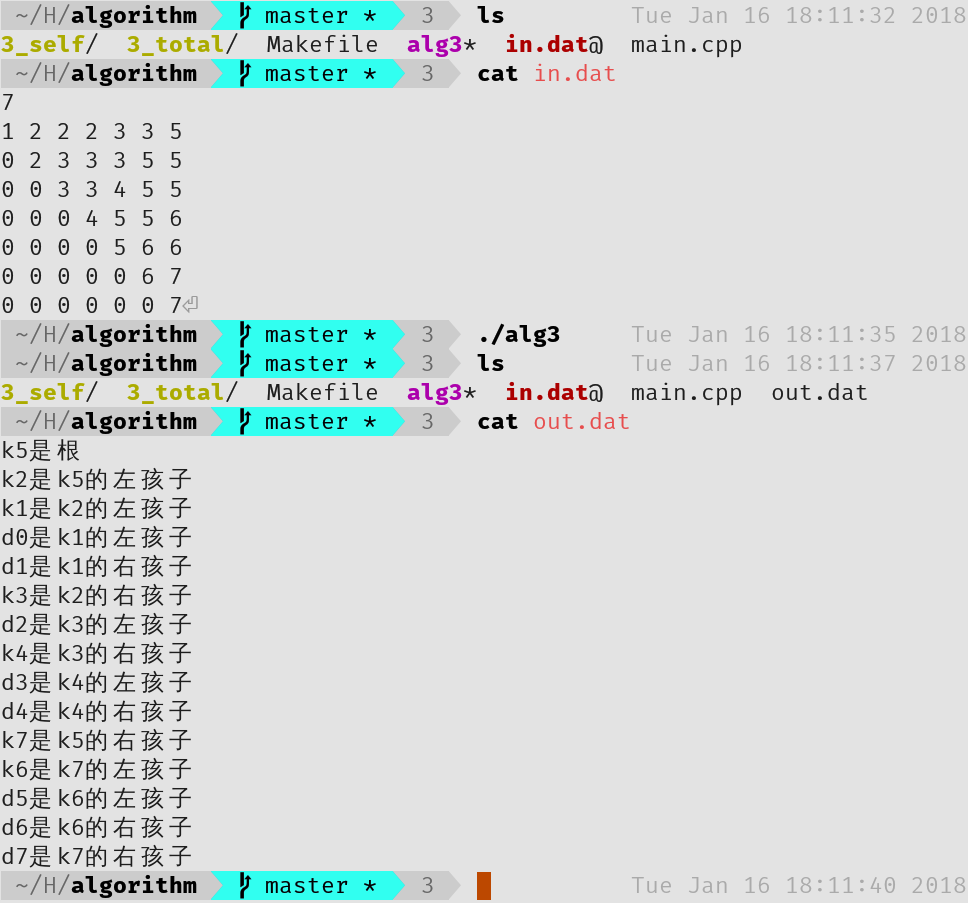
\includegraphics[width=0.65\linewidth]{result3.png}
    \caption{测试过程以及结果}
    \label{fig:result3}
\end{figure}

\section{技术总结}
\label{sec:ji_zhu_zong_jie_3}
在通过$root$矩阵对于原二叉搜索树的构建过程中,只有了解了$root$矩阵是如何生成的才能够逆推原有的搜索树结构。此外,在此算法中对于左孩子和右孩子递归调用的顺序以及递归的停止调教是十分重要的。若不能够正确的处理这些问题则会输出错误的结果。

% Chapter Four %%%%%%%%%%%%%%
%%%%%%%%%%%%%%%%%%%%%%%%%%%%%
\chapter{Floyd Warshell最短路径算法}
\label{cha:floyd_warshellzui_duan_lu_jing_suan_fa_}

\section{题目描述}
\label{sec:ti_mu_miao_shu_4}
补充 ALL-PATHS算法,增加前驱矩阵(Chp.25.2),使得在求出结点间的最短路径长度矩阵A后,能够推导出每对结点间的最短路径。
\begin{itemize}
    \item 输入文件:in.dat
        \begin{itemize}
            \item 格式:第一行为一个整数,表示测试用例的组数,其后跟相应组数的测试用例
            \item 每组测试用例包括:
                \begin{itemize}
                    \item 首行:一个整数,表示本组测试用例包含的结点数 n,其后跟 n 行
                    \item 其后:每行$n$个整数,表示结点间邻接关系及边的长度(邻接成本矩阵)。边的长度<100, 100 即表示结点间没有边。
                \end{itemize}
        \end{itemize}
    \item 输出文件:out.dat
        \begin{itemize}
            \item 格式:第一行为一个整数,表示测试用例的组数,其后跟相应组数的测试用例
            \item 每组测试用例输出包括:
                \begin{itemize}
                    \item 首行:一个整数,表示本组测试用例包含的结点数$n$,其后跟$n+n^2$行
                    \item 其后:开始的$n$数,表示结点间最短路径的长度(A 矩阵)。路径的程度<32767, 32767 即表示结点间没有可达的路径。其后 n2 行,顺次输出结点对(1,1)、 (1,2)、 ...、 (1,n), (2,1)、 (2,2)、 ...、(2,n)、...(n,1)、...、(n,n)之间的最短路径结点序列,结点间用空格隔开。(i,i)输出 i,若(i,j)之间没有路径,输出 NULL。
                \end{itemize}
        \end{itemize}
\end{itemize}

\section{算法设计}
\label{sec:suan_fa_she_ji_4}
ALL-PATHS算法实现的是Floyd-Warshall算法,其原理是动态规划。令$D_{i,j,k}$为从$i$到$j$的只以$(1, 2, \ldots , k)$中的节点为中间节点的最短路径的长度,那么
\begin{equation}
    \label{eq:d}
    D_{i,j,k}=\left\{
        \begin{array}{l l}
            D_{i,j,k}=D_{i,j,k-1}+D_{k,j,k-1} & , \text{最短路径经过点}k \\
            D_{i,j,k}=D_{i,j,k-1} & , \text{若最短路径不经过点}k
        \end{array}
    \right.
\end{equation}

因此$D_{i,j,k}=\min\{D_{i,j,k-1}, D_{i,k,k-1}+D_{k,j,k-1}\}$。\par
但是Floyd-Warshall算法只能给出任意两点间最短路径的长度而不能给出具体的路径。要使其能够得到具体的路径,需要前驱矩阵$\Pi$来存储最短路径树。令$\pi_{ij}^{(k)}$为从节点$i$到节点$j$的一条在所有中间节点都取自集合${1, 2, \ldots, k}$的最短路径上$j$的前驱节点,那么对于任意两个节点$m, n$就可以通过从$\pi_{mn}$开始查询$\Pi$直到查询完整个路径来构建从$m$到$n$的最短路径。而对于$k\geq 1$,

\begin{equation}
    \label{eq:pi}
    \pi_{i,j}^{(k)}=\left\{
        \begin{array}{l l}
            \pi_{ij}^{(k-1)} & , d_{ij}^{(k-1)} \leq d_{ik}^{(k-1)} + d_{kj}^{(k-1)}\\
            \pi_{kj}^{(k-1)} & , d_{ij}^{(k-1)} > d_{ik}^{(k-1)} + d_{kj}^{(k-1)}
        \end{array}
    \right.
\end{equation}

于是通过公式\ref{eq:d}和公式\ref{eq:pi}可以得到扩展过后的ALL-PATHS算法如下:
\begin{simpleAlgorithm}{最短路径构建算法}
    \Procedure{AllPaths}{$W$}
    \State $dist \gets |V|\times |V|$ array of $\infty$ \Comment{$dist$为最短路径表$D$}
    \State $next \gets |V|\times |V|$ array of $nil$ \Comment{$next$为前驱子矩阵$\Pi$}
    \For{each edge (u, v)} \Comment{初始化$D$和$\Pi$}
        \State $dist[u, v] \gets W(u, v)$ \Comment{边$(u, v)$的权重}
        \State $next[u, v] \gets v$
    \EndFor
    \For{$k=1$ to $|V|$}  \Comment{扩展的Floyd-Warshall算法}
        \For{$i=1$ to $|V|$}
            \For{$j=1$ to $|V|$}
                \If{$dist[i,j] > dist[i,k]+dist[k,j]$}
                    \State $dist[i,j] \gets dist[i,k] + dist[k,j]$
                    \State $next[i,j] \gets next[i,k]$
                \EndIf
            \EndFor
        \EndFor
    \EndFor
    \For{$i=1$ to $|V|$} \Comment{构造最短路径}
        \For{$j=1$ to $|V|$}
            \If{$next[u,v]=nil$}
                \State continue
            \EndIf
            \State $path[i,j] = [i]$
            \While{$i \neq j$}
                \State $i \gets next[i][j]$
                \State $path[i,j]$.append($i$)
            \EndWhile
        \EndFor
    \EndFor
    \State \Return $path$, $dist$
    \EndProcedure
\end{simpleAlgorithm}

在算法中,首先运行Floyd-Warshall算法,在运行时同时构造$D$和$\Pi$两个矩阵,在此算法运行完成后,通过$\Pi$矩阵求出每一个点对之间的路径,然后将结果返回给调用者进行输出。\par

程序的流程图如\ref{fig:flowchart4}所示,首先,通过使用Floyd-Warshall算法,找出每两个点对之间的最短路径的同时构建$\Pi$矩阵,在这一步骤完成后对于所有点对$(u,v)$在上一步得到的$\Pi$矩阵中找到最短路径,最后把得到的结果返回给上层进行输出(流程图中未给出)。需要注意的是,在算法开始前需要正确的初始化$D$和$\Pi$,否则不能够得到正确答案。

\begin{figure}[ht]
    \centering
    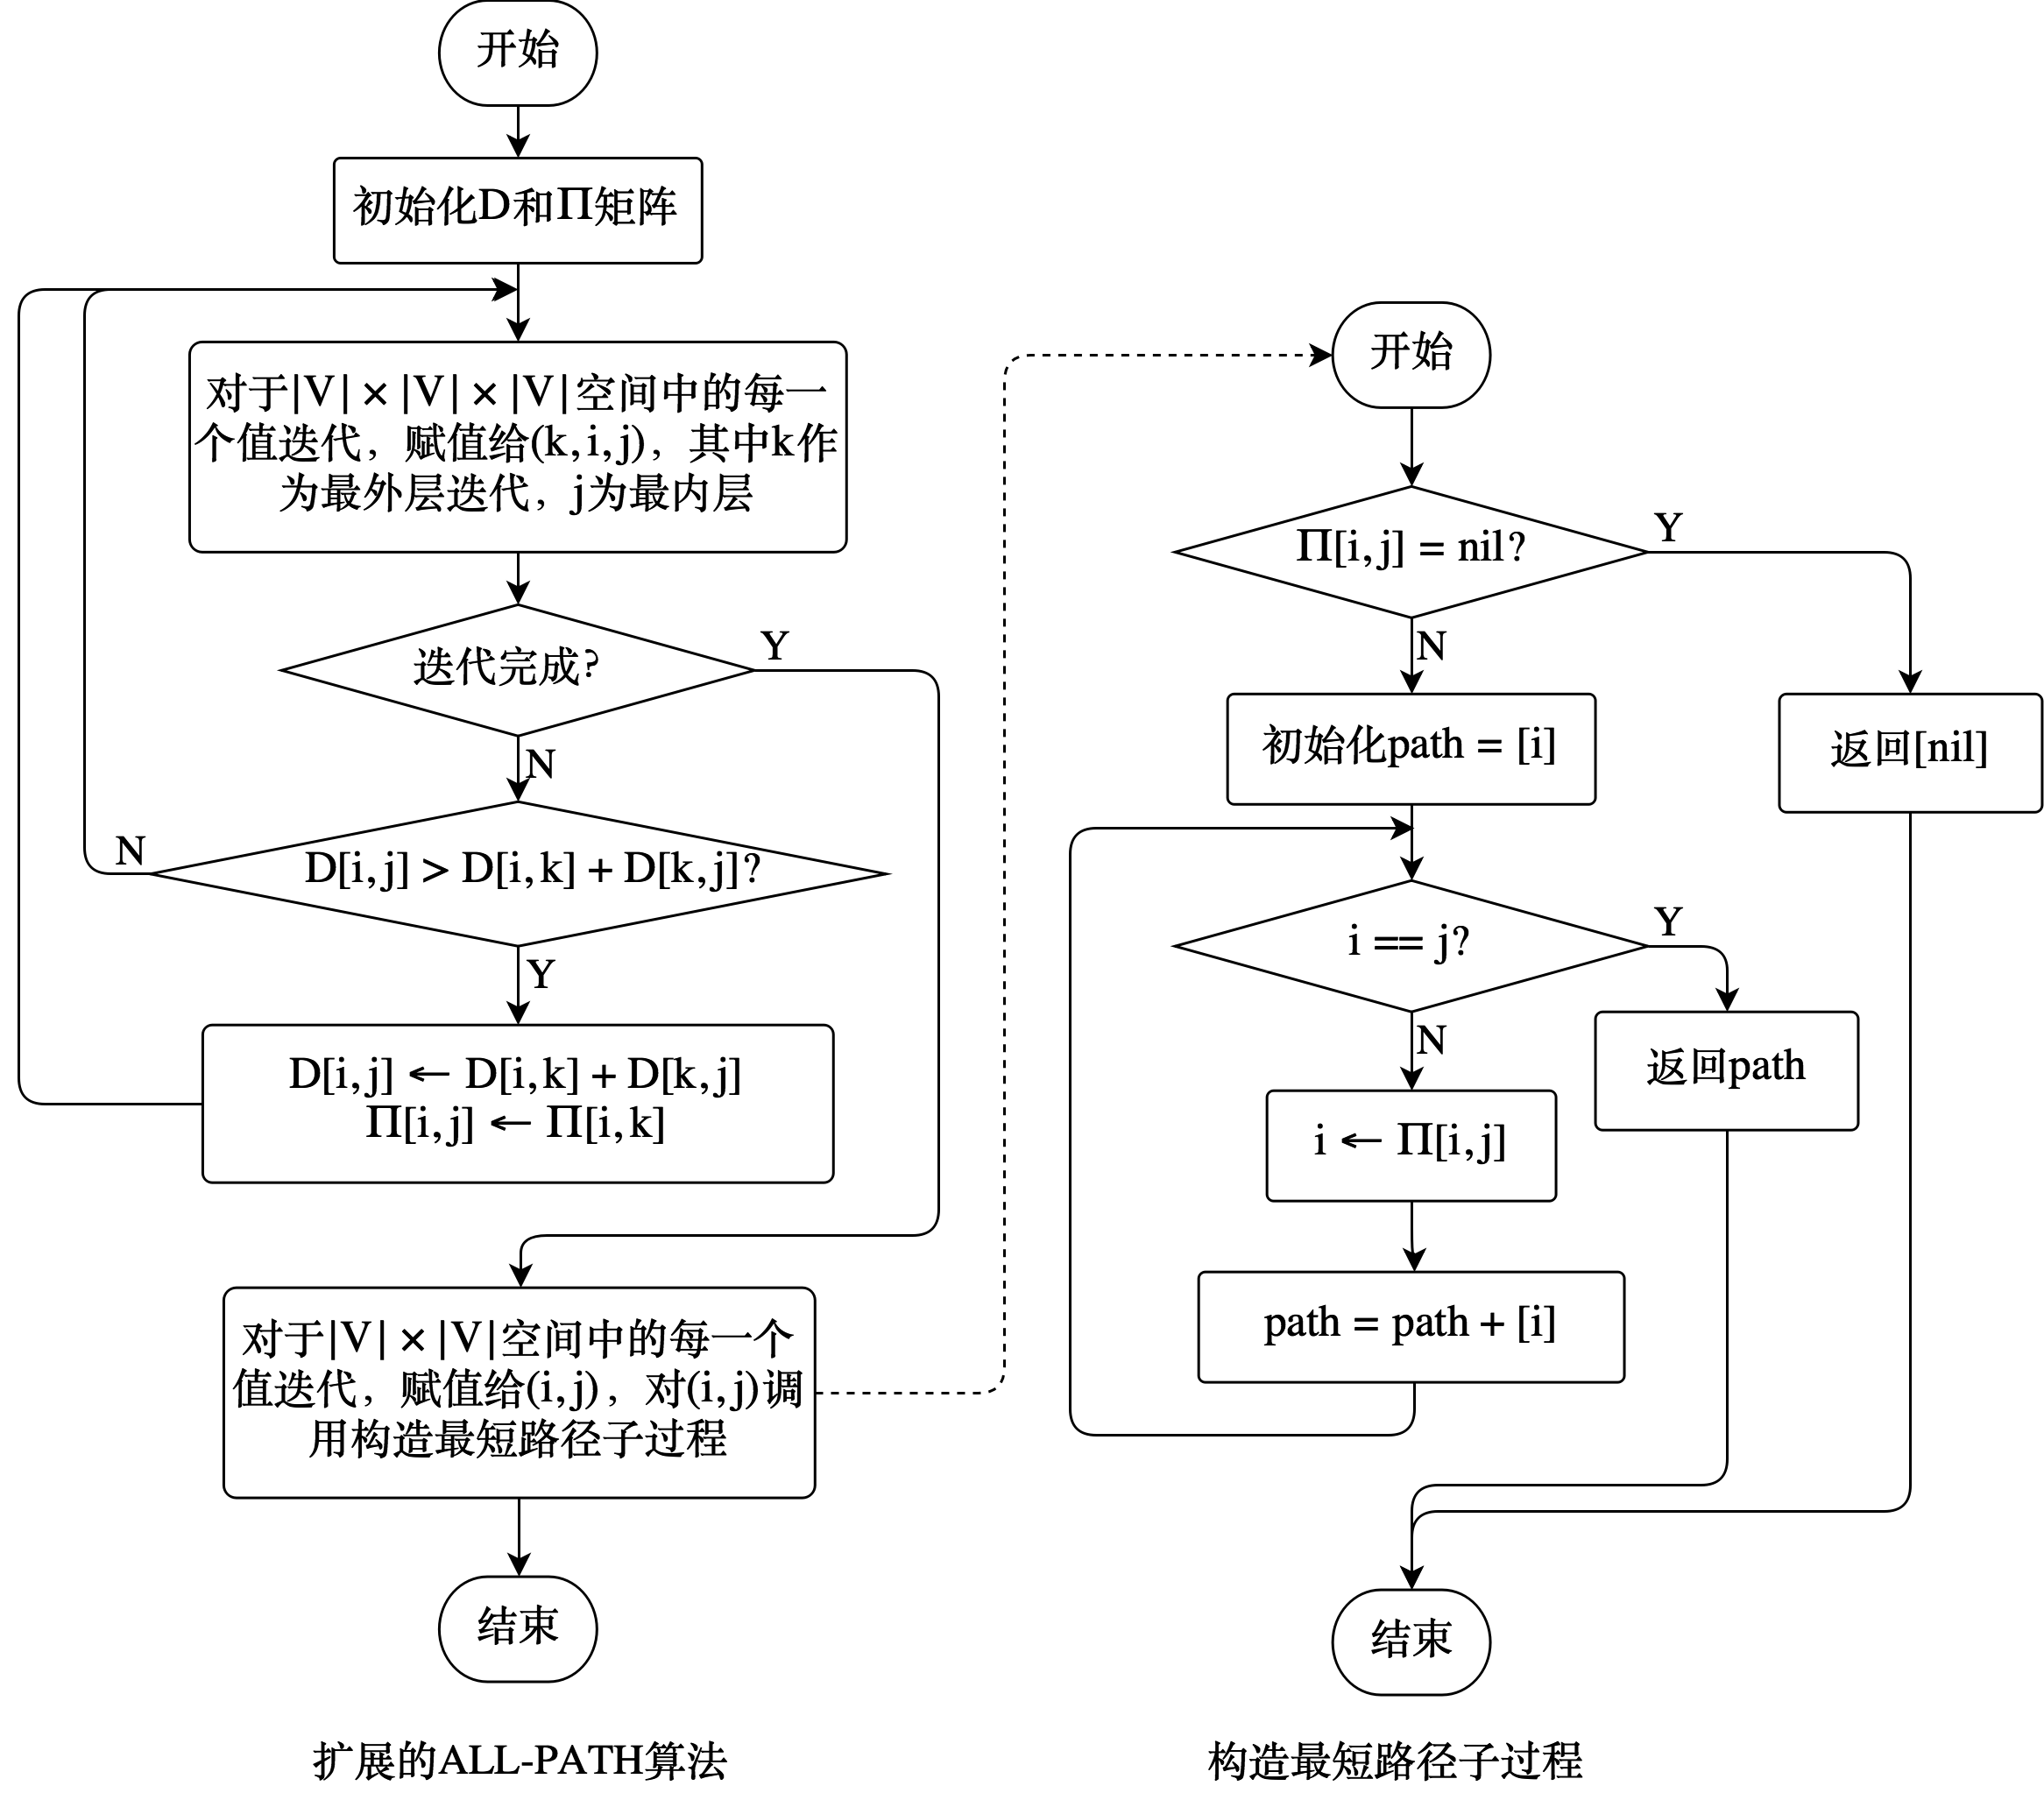
\includegraphics[width=0.8\linewidth]{flowchart4.png}
    \caption{程序流程图}
    \label{fig:flowchart4}
\end{figure}

\section{测试分析}
\label{sec:ce_shi_fen_xi_4}
对于给定的in.dat运行编译好的程序,in.dat对应的拓扑图如\ref{fig:description4}所示,in.dat的内容、运行的过程以及输出的out.dat中的结果如\ref{fig:result4}所示。从图中可以看出,程序能够正确的生成out.dat,并且输出结果与预期结果一致。

\begin{figure}[H]
    \centering
    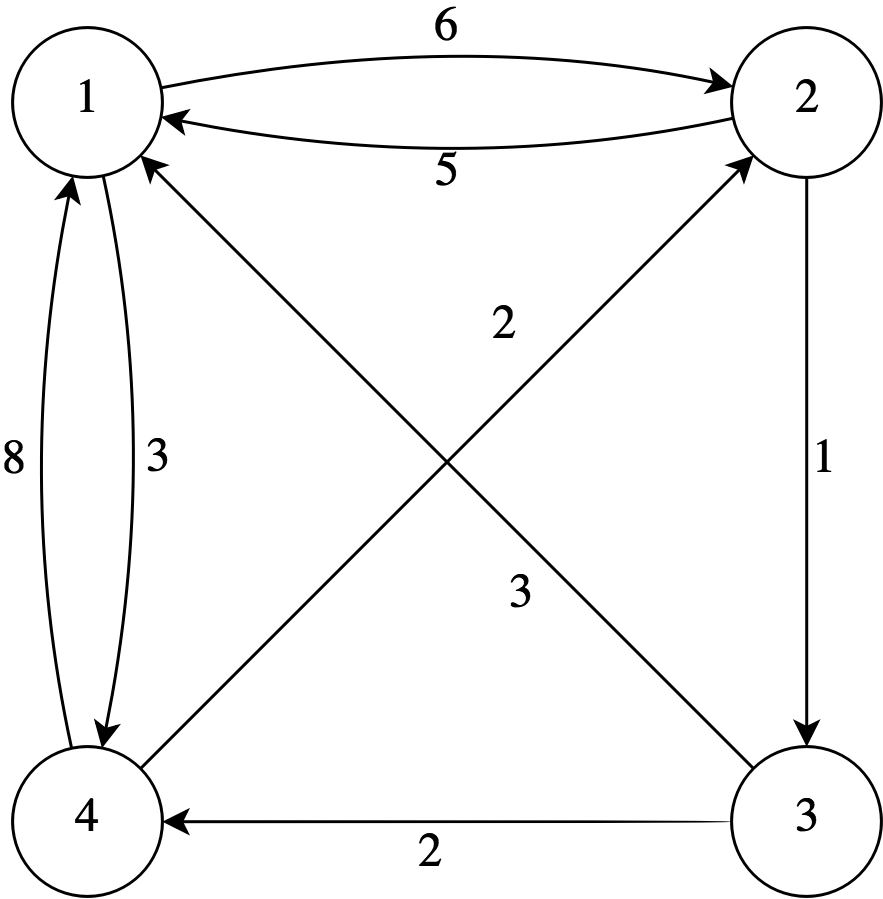
\includegraphics[width=0.3\linewidth]{description4.png}
    \caption{数据对应的拓扑图}
    \label{fig:description4}
\end{figure}

\begin{figure}[ht]
    \centering
    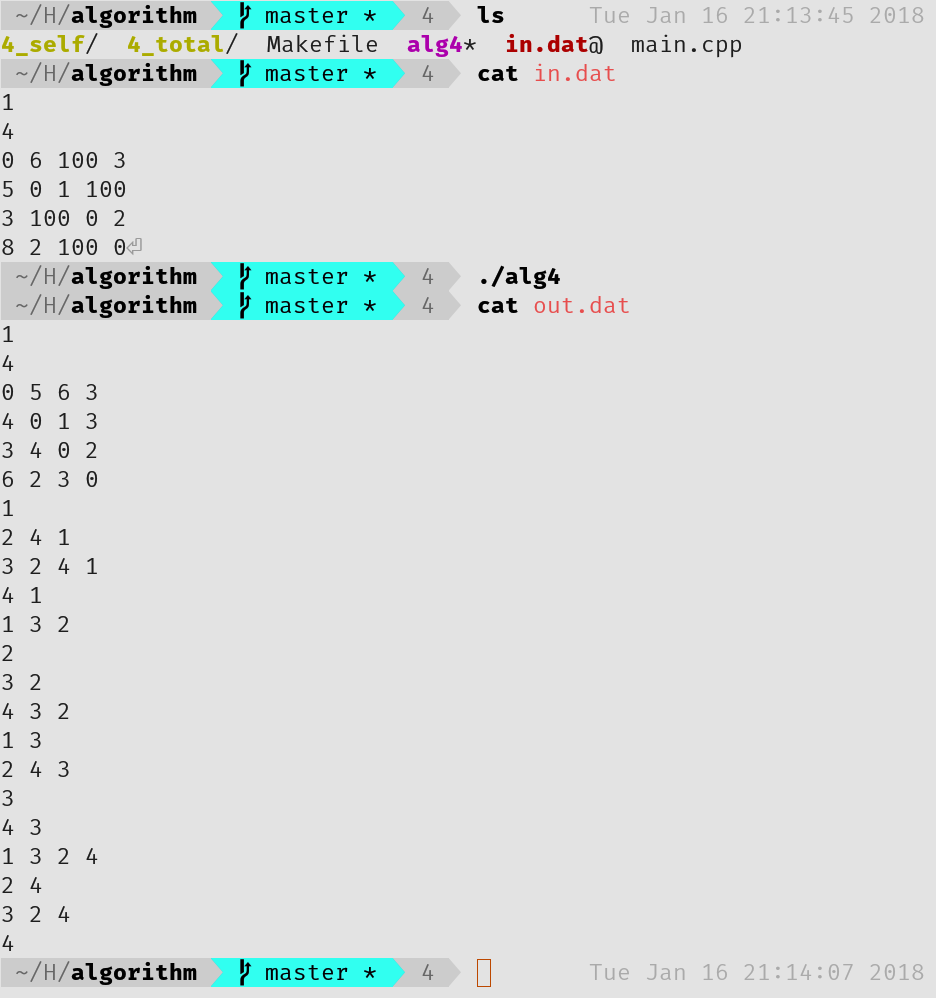
\includegraphics[width=0.8\linewidth]{result4.png}
    \caption{测试过程以及输出结果}
    \label{fig:result4}
\end{figure}

\section{技术总结}
\label{sec:ji_zhu_zong_jie_4}
构建最短路径的关键技术是前驱矩阵$\Pi$的生成,只要能够生成前去矩阵$\Pi$,就可以通过依次迭代的方法找到任意两点之间的最短路径,此外,本程序还采用了直接在原来的矩阵上进行迭代的技术,从而使空间复杂度从$O(N^3)$下降到了$O(N^2)$。在直接在原有空间上进行迭代时需要注意不能够把将来还需要使用的值覆盖掉,即需要特别注意迭代的顺序,以保证结果的正确性。\par

% Chapter Five %%%%%%%%%%%%%%
%%%%%%%%%%%%%%%%%%%%%%%%%%%%%
\chapter{Wooden Sticks (POJ 1065)}
\label{cha:wooden_sticks_poj_1065_}

\section{题目描述}
\label{sec:ti_mu_miao_shu_5}

\subsection{Description}
There is a pile of n wooden sticks. The length and weight of each stick are known in advance. The sticks are to be processed by a woodworking machine in one by one fashion. It needs some time, called setup time, for the machine to prepare processing a stick. The setup times are associated with cleaning operations and changing tools and shapes in the machine. The setup times of the woodworking machine are given as follows:\par

\begin{itemize}
    \item The setup time for the first wooden stick is 1 minute.
    \item Right after processing $a$ stick of length $l$ and weight $w$ , the machine will need no setup time for a stick of length $l'$ and weight $w'$ if $l \leq l'$ and $w \leq w'$. Otherwise, it will need 1 minute for setup.
\end{itemize}

You are to find the minimum setup time to process a given pile of n wooden sticks. For example, if you have five sticks whose pairs of length and weight are (9,4), (2,5), (1,2), (5,3), and (4,1), then the minimum setup time should be 2 minutes since there is a sequence of pairs (4,1), (5,3), (9,4), (1,2), (2,5) .\par

\subsection{Input}
The input consists of T test cases. The number of test cases (T) is given in the first line of the input file. Each test case consists of two lines: The first line has an integer $n$ , $1 \leq n \leq 5000$ , that represents the number of wooden sticks in the test case, and the second line contains $2n$ positive integers $l_1, w_1, l_2, w_2, ..., l_n, w_n$, each of magnitude at most 10000 , where $l_i$ and $w_i$ are the length and weight of the $i$ th wooden stick, respectively. The $2n$ integers are delimited by one or more spaces. \par

\subsection{Output}
The output should contain the minimum setup time in minutes, one per line. \par

\subsection{Sample Input}
\begin{lstlisting}
3
5
4 9 5 2 2 1 3 5 1 4
3
2 2 1 1 2 2
3
1 3 2 2 3 1
\end{lstlisting}

\subsection{Sample Output}
\begin{lstlisting}
2
1
3
\end{lstlisting}

\section{算法设计}
\label{sec:suan_fa_she_ji_5}
首先将所有的木棍按照重量进行排序,然后按照长度进行排序(均为稳定排序),排序完成后所有的木棍就是按照长度排序好的非降序序列,且当长度相等时是按照重量排好的非降序序列。然后求出这一序列对于重量的最长下降子序列的长度,就是所得到的结果。\par

\textbf{证明:}假设上述最长下降子序列的长度为$m$,根据木棍的排列规则可知这下降子序列中的木棍的长度不可能相等(由于长度相等时重量是按照非降序进行排序的),因此这一最长下降子序列中的任意两个木棍$i,j$都满足$l_i<l_j$且$w_i>w_j$,此时它们两两``不兼容''(不可能位于同一个对于长度和重量而言都是非降序的子序列中)。因此所花费的费用至少为$m$。\par

使用贪心算法,维护一个当前所有非降子序列中最后一个值的列表M,然后对于排好序的木棍进行依次进行迭代,每一次迭代首先观察其长度和重量是否都大于M中的某一个木棍的对应值,若是,更新该木棍的对应值,将这一木棍的属性插入列表末尾,最后得到的列表的长度就是最长下降子序列的长度m(可用剪切-粘贴法证明如果不按照这一规则构建M则M的长度将会大于或等于m),因此能够在花费为$m$的情况下处理所有的木棍。又已知话费至少为$m$,因此$m$即为问题的解。求解的算法如下:\par

\begin{simpleAlgorithm}{Wooden Sticks问题求解算法}
    \Procedure{WoodenSticks}{$S$} \Comment{$S$为所有木棍\{长度,重量\}的列表}
    \State \Call{StableSort}{$S, weight$} \Comment{按照重量稳定排序}
    \State \Call{StableSort}{$S, length$} \Comment{按照长度稳定排序}
    \State $M \gets \{\}$
    \For{$stick$ in $S$}
        \If{$stick.weight \geq \min\{s.weight | s \in M\}$}
            \State $s \gets \max\{s | s \in M \bigwedge s.weight < stick.weight\}$
            \State $s \gets stick$
        \Else
            \State $S$.append($stick$)
        \EndIf
    \EndFor
    \State \Return $S.length$
    \EndProcedure
\end{simpleAlgorithm}

这一算法的流程图如\ref{fig:flowchart5}所示,首先,也是最重要的一步:对于重量和长度进行稳定排序,以构建一个首先按照长度然后按照重量的费降序序列。然后对于这一序列中的每一个木棍进行迭代,如果木棍的重量大于$M$中的重量最小的木棍的重量,那么更新列表中比这一木棍重量小的木棍中重量最大的那个为当前的木棍。

\begin{figure}[ht]
    \centering
    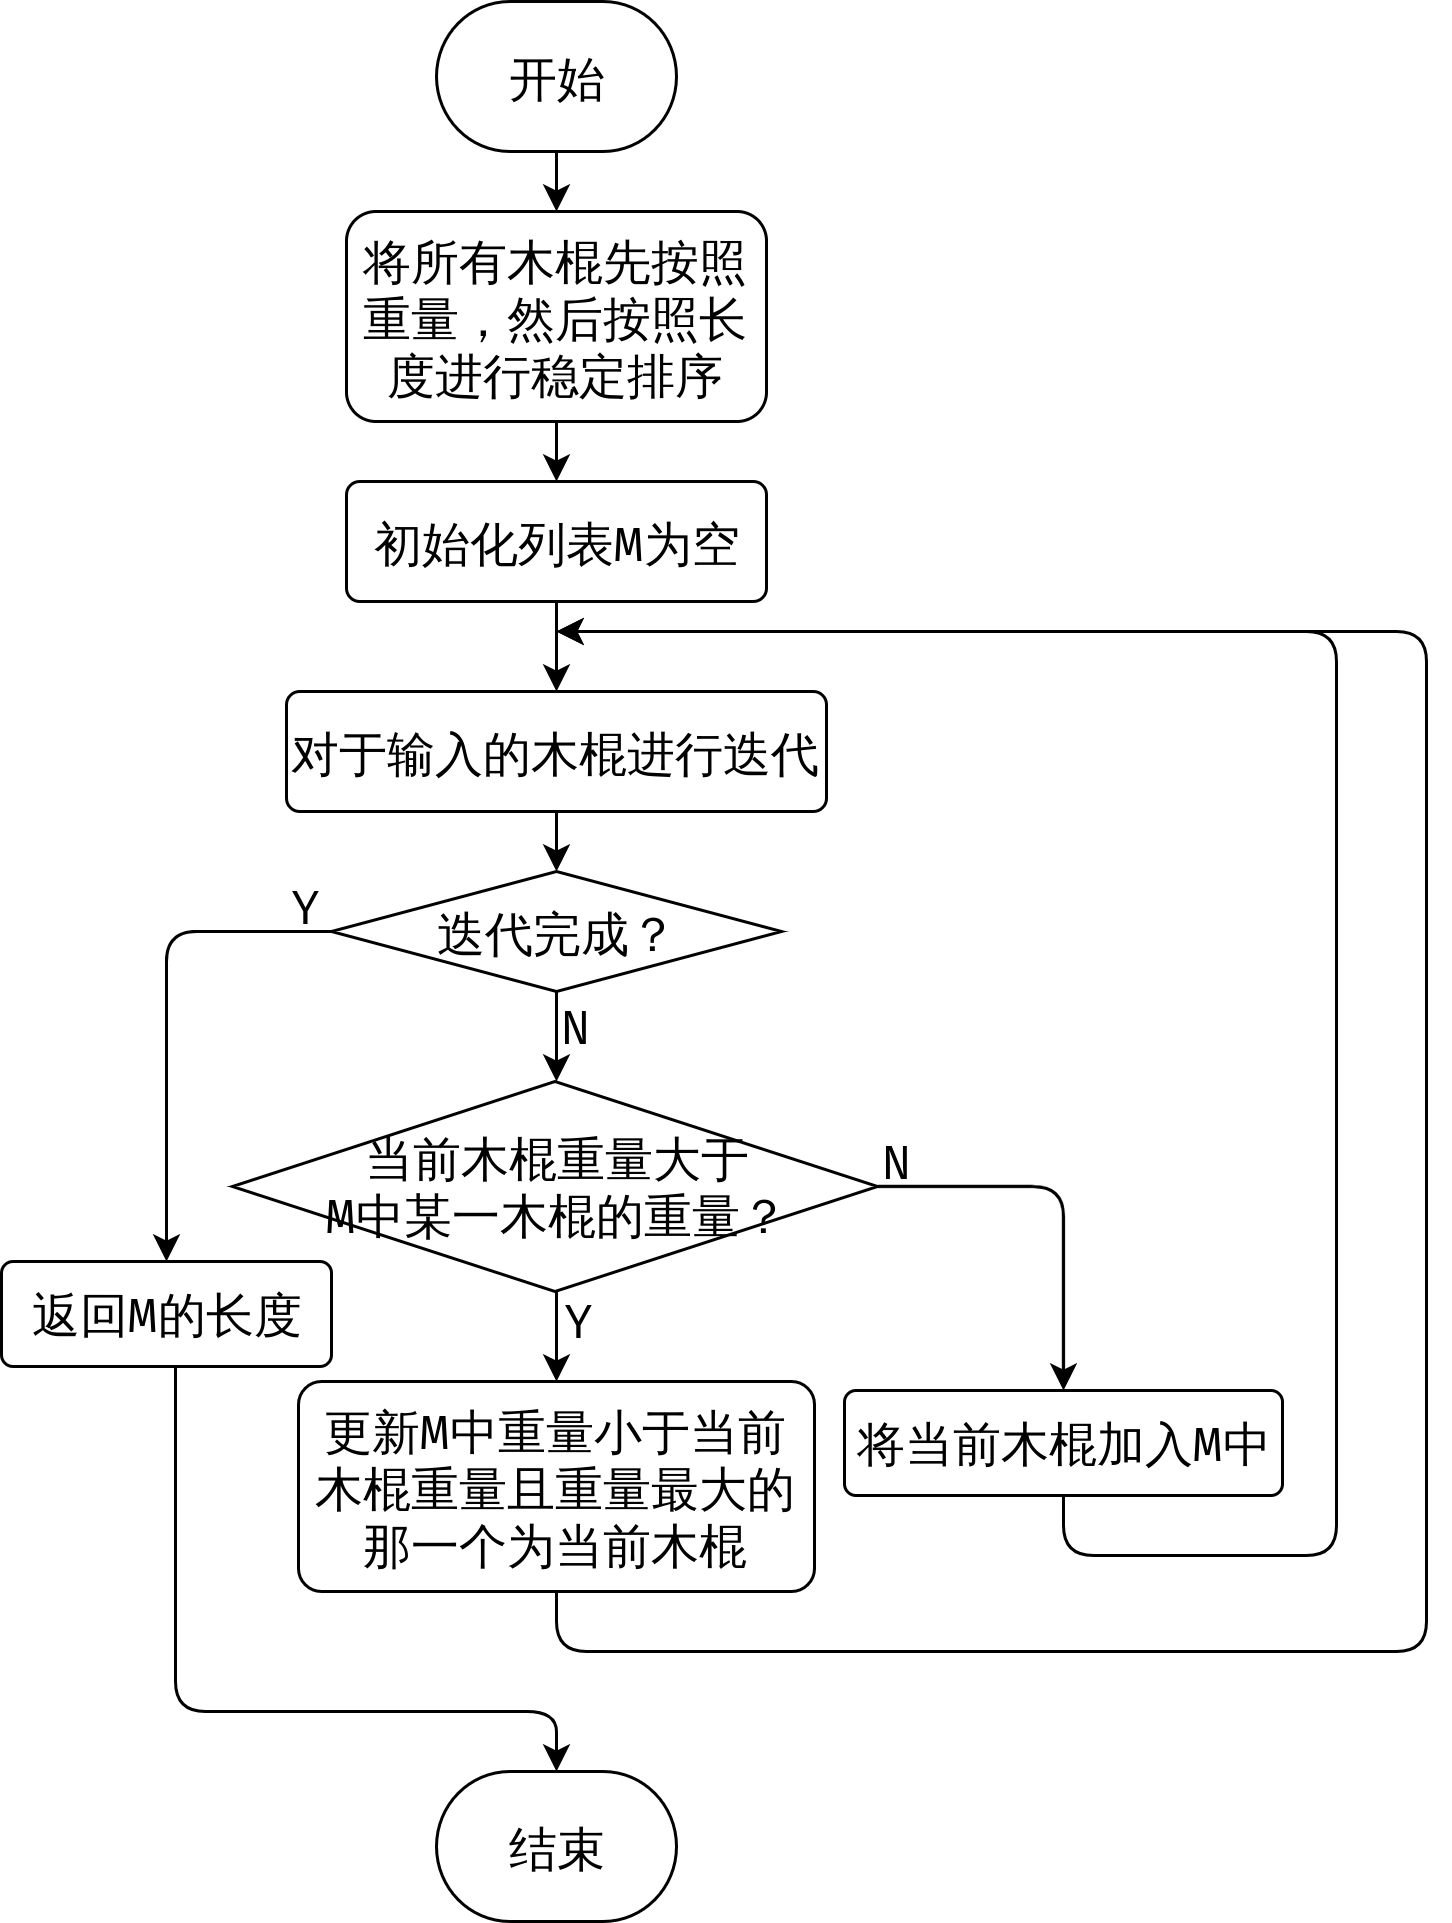
\includegraphics[width=0.5\linewidth]{flowchart5.png}
    \caption{程序流程图}
    \label{fig:flowchart5}
\end{figure}

\section{测试分析}
\label{sec:ce_shi_fen_xi_5}
如\ref{fig:result5}所示,对于POJ提供的测试用例,程序在47MS内全部通过,由此可以说明程序运行正确。

\begin{figure}[ht]
    \centering
    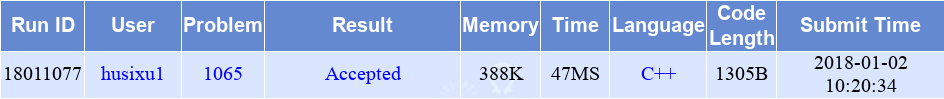
\includegraphics[width=0.9\linewidth]{result5.png}
    \caption{POJ测试结果}
    \label{fig:result5}
\end{figure}

\section{技术总结}
\label{sec:ji_zhu_zong_jie_5}
对于这一问题而言,使用稳定排序以及贪心算法是至关重要的。如果不适用稳定排序可能则不能保证生成先按照长度非降序再按照重量非降序的序列,对于降序最长子序列的统计而言,使用贪心算法则可以在保证答案正确的情况下减少所需要的时间。

% Chapter Six %%%%%%%%%%%%%%%
%%%%%%%%%%%%%%%%%%%%%%%%%%%%%
\chapter{Gone Fishing (POJ 1042)}
\label{cha:gone_fishing_poj_1042_}

\section{题目描述}
\label{sec:ti_mu_miao_shu_6}

\subsection{Description}
John is going on a fishing trip. He has $h$ hours available $(1 \leq h \leq 16)$, and there are n lakes in the area $(2 \leq n \leq 25)$ all reachable along a single, one-way road. John starts at lake 1, but he can finish at any lake he wants. He can only travel from one lake to the next one, but he does not have to stop at any lake unless he wishes to. For each $i = 1, \ldots, n - 1$, the number of 5-minute intervals it takes to travel from lake $i$ to lake $i + 1$ is denoted $t_i (0 < t_i \leq 192)$. For example, $t_3 = 4$ means that it takes 20 minutes to travel from lake 3 to lake 4. To help plan his fishing trip, John has gathered some information about the lakes. For each lake $i$, the number of fish expected to be caught in the initial 5 minutes, denoted $f_i (f_i \geq 0)$, is known. Each 5 minutes of fishing decreases the number of fish expected to be caught in the next 5-minute interval by a constant rate of $d_i (di \geq 0)$. If the number of fish expected to be caught in an interval is less than or equal to $d_i$ , there will be no more fish left in the lake in the next interval. To simplify the planning, John assumes that no one else will be fishing at the lakes to affect the number of fish he expects to catch. \par

Write a program to help John plan his fishing trip to maximize the number of fish expected to be caught. The number of minutes spent at each lake must be a multiple of 5. \par

\subsection{Input}
You will be given a number of cases in the input. Each case starts with a line containing $n$. This is followed by a line containing $h$. Next, there is a line of n integers specifying $f_i (1 \leq i \leq n)$, then a line of n integers $d_i (1 \leq i \leq n)$, and finally, a line of n - 1 integers $t_i (1 \leq i \leq n - 1)$. Input is terminated by a case in which $n = 0$.\par

\subsection{Output}
\label{sub:output}
For each test case, print the number of minutes spent at each lake, separated by commas, for the plan achieving the maximum number of fish expected to be caught (you should print the entire plan on one line even if it exceeds 80 characters). This is followed by a line containing the number of fish expected. \par
If multiple plans exist, choose the one that spends as long as possible at lake 1, even if no fish are expected to be caught in some intervals. If there is still a tie, choose the one that spends as long as possible at lake 2, and so on. Insert a blank line between cases.

\subsection{Sample Input}
\begin{lstlisting}
2
1
10 1
2 5
2
4
4
10 15 20 17
0 3 4 3
1 2 3
4
4
10 15 50 30
0 3 4 3
1 2 3
0
\end{lstlisting}

\subsection{Sample Output}
\begin{lstlisting}
45, 5
Number of fish expected: 31

240, 0, 0, 0
Number of fish expected: 480

115, 10, 50, 35
Number of fish expected: 724
\end{lstlisting}

\section{算法设计}
\label{sec:suan_fa_she_ji_6}
对于题目进行分析,发现若能够知道John最终停止湖$k$,那么他最终旅行的时间是固定的,为$\sum_{i=1}^{k-1}t_i$,从总时间中减去这段时间后,可以看做John可以在湖$[1, k]$之间随意的移动而不需要花费时间,最终只需统计在每个湖上花费的总时间$total_i$然后在湖$i$上花费$total_i$这么长的时间即可。\par
因此将旅行所用的时间减去后,剩下的时间可以使用贪心算法,在每一个5分钟选择湖$[1, k]$中收益最大的那个,并花费5分钟在其上钓鱼即可。如果在某个5分钟时间段内两个或多个湖收益相等且最大,那么选择其中编号最小的进行处理。\par
对于每一个给定的湖的树龄$n$,对于每一个可能的$k$运行上述算法,然后取能够取得的最好的结果返回即可。具体算法如下:\par
\begin{simpleAlgorithm}{GoneFishing问题求解算法}
    \Procedure{GoneFishing}{$F, D, T, h$} \Comment{$F=\{f_i\}, D=\{d_i\}, T=\{t_i\}$}
    \State $bestPath \gets []$
    \State $bestResult \gets -1$
    \For{k=1 to n}
        \State $m = h * 60 - \sum_{1}^{k-1}t_i$  \Comment{能够用于钓鱼的分钟数}
        \State $rResult \gets 0$ \Comment{当前$k$值下的最佳结果}
        \State $rPath \gets [0]\times k$\Comment{当前$k$值下的最佳路径}
        \While{$m \neq 0$}
        \State $i \gets \min\{i | i \in [1,k] \bigwedge f_i \geq f_j, \forall j \in [1,k] \}$
            \State $rResult \gets rResult + f_i$
            \State $rPath[i] \gets rPath[i] + 5$
            \State $f_i \gets \max\{f_i - d_i, 0\}$
            \State $m \gets m-5$
        \EndWhile
        \If{$rResult > bestResult$}
            \State $bestPath \gets rPath$
            \State $bestResult \gets rResult$
        \EndIf
    \EndFor
    \State \Return $bestPath, bestResult$
    \EndProcedure
\end{simpleAlgorithm}

\begin{figure}[ht]
    \centering
    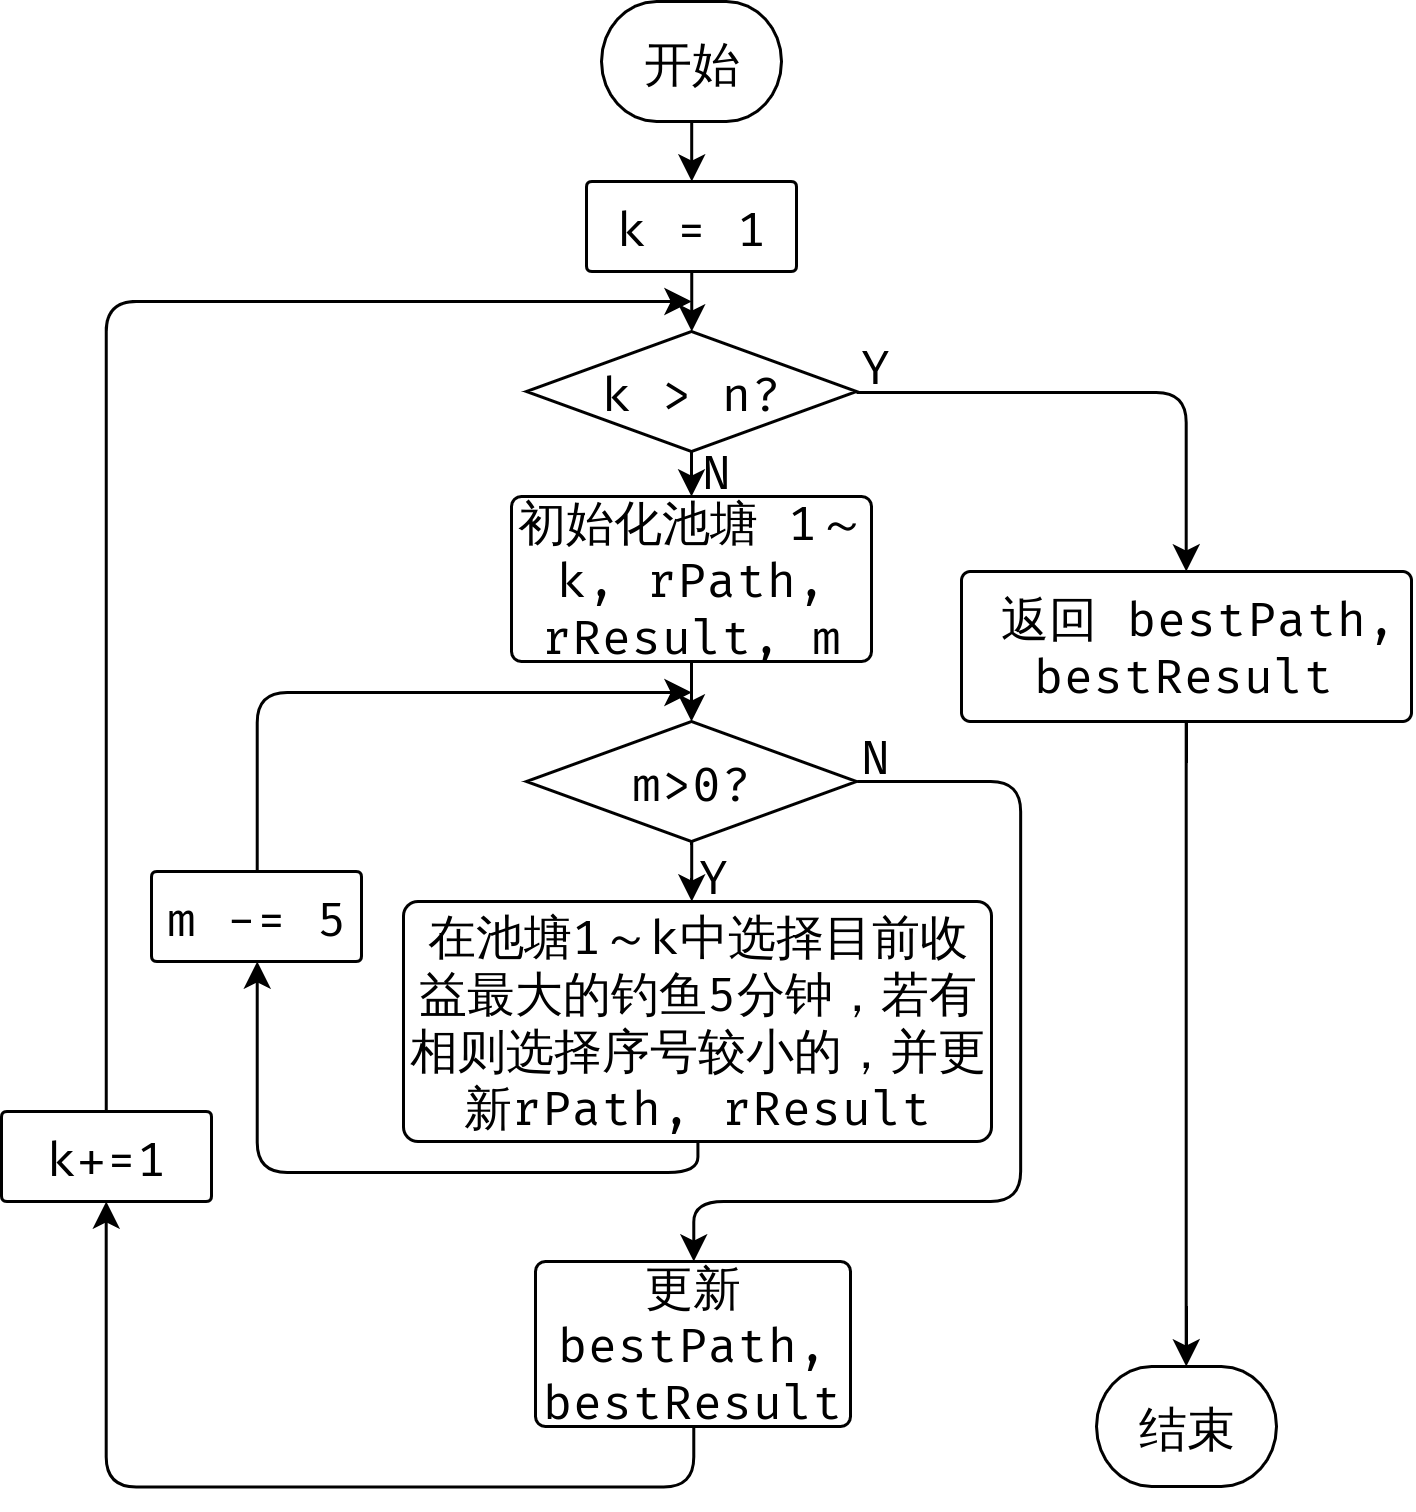
\includegraphics[width=0.42\linewidth]{flowchart6.png}
    \caption{程序流程图}
    \label{fig:flowchart6}
\end{figure}

与设计中预想的一样,在算法中,首先对于每一个可能的k值进行枚举,从总的时间中减去旅行所用的时间后每次选取收益最大的池塘在上面钓鱼即可,流程图如图\ref{fig:flowchart6}所示。

\section{测试分析}
\label{sec:ce_shi_fen_xi_6}
如\ref{fig:result6}所示,对于POJ提供的测试用例,程序在188MS内全部通过,由此可以说明程序运行正确。

\begin{figure}[ht]
    \centering
    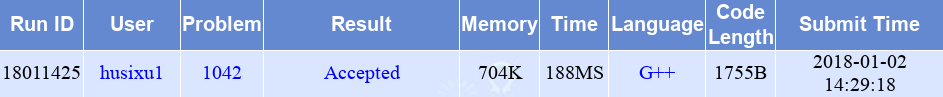
\includegraphics[width=0.9\linewidth]{result6.png}
    \caption{POJ测试结果}
    \label{fig:result6}
\end{figure}

\section{技术总结}
\label{sec:ji_zhu_zong_jie_6}
对于``Each 5 minutes of fishing decreases the number of fish expected to be caught in the next 5-minute interval'' 这句话的理解应该是:如果不在该lake上面钓鱼,那么该lake里面的鱼是不会减少的,只有当选择了该lake,那么鱼会稳定减少直至为0。此外,使用贪心算法也是能够快速的结束这道题的关键。

% Chapter Seven %%%%%%%%%%%%%
%%%%%%%%%%%%%%%%%%%%%%%%%%%%%
\chapter{Corn Field (POJ 3254)}
\label{cha:corn_field_poj_3254_}

\section{题目描述}
\label{sec:ti_mu_miao_shu_7}

\subsection{Description}
Farmer John has purchased a lush new rectangular pasture composed of $M$ by $N (1 \leq M \leq 12; 1 \leq N \leq 12)$ square parcels. He wants to grow some yummy corn for the cows on a number of squares. Regrettably, some of the squares are infertile and can't be planted. Canny FJ knows that the cows dislike eating close to each other, so when choosing which squares to plant, he avoids choosing squares that are adjacent; no two chosen squares share an edge. He has not yet made the final choice as to which squares to plant.\par

Being a very open-minded man, Farmer John wants to consider all possible options for how to choose the squares for planting. He is so open-minded that he considers choosing no squares as a valid option! Please help Farmer John determine the number of ways he can choose the squares to plant.

\subsection{Input}
Line 1: Two space-separated integers: $M$ and $N$ \par
Lines 2...M+1: Line i+1 describes row i of the pasture with $N$ space-separated integers indicating whether a square is fertile (1 for fertile, 0 for infertile)\par

\subsection{Output}
Line 1: One integer: the number of ways that FJ can choose the squares modulo 100,000,000.\par

\subsection{Sample Input}
\begin{lstlisting}
2 3
1 1 1
0 1 0
\end{lstlisting}

\subsection{Sample Output}
\begin{lstlisting}
9
\end{lstlisting}

\subsection{Hint}
Number the squares as follows:\par
\begin{lstlisting}
    1 2 3
      4
\end{lstlisting}

There are four ways to plant only on one squares (1, 2, 3, or 4), three ways to plant on two squares (13, 14, or 34), 1 way to plant on three squares (134), and one way to plant on no squares. 4+3+1+1=9.

\section{算法设计}
\label{sec:suan_fa_she_ji_7}
由于$1\leq N\leq 12$,并且每一片田只可能有能种草和不能种草两种属性,因此可以使用状态压缩。使用一张长为$M$表$I$来表示这是否为不肥沃的,这样直接用每一行的田地属性与种草状态进行与操作,若不为0则表示这是一种非法状态。\par
考虑玩状态压缩后考虑题目的求解方法。使用动态规划的方法,使用一张$M\times 2^N$的表$D$,其中$D[i,j]$表示当第$i$行状态为$j$时由多少种可行的方法。显然,当$j\&I[i]$时是非法状态,此时$D[i,j]$应该为0,否则$D[i,j]$应该为上一行所有与之不发生冲突的状态的可能性之和。因此可以得到:
\[
    D[i,j]=\left\{
        \begin{array}{l l}
            0 & , j\&I[i] \neq 0 \\
            \sum\limits_{k\&j=0} D[i-1, k] & , j\&I[i] = 0
        \end{array}
    \right.
\]

然后根据此状态转移方程依次对于$D$中的每一行进行迭代即可。最终的结果就是D中最后一行的和$\sum_{k=1}^{2^N}D[M, k]$。第一行的初始状态应该为:
\[
    D[1, j]=\left\{
        \begin{array}{l l}
            0 & , j\&I[1] \neq 0 \\
            1 & , j\&I[1] = 0 \\
        \end{array}
    \right.
\]
依照初始状态以及状态转移方程的算法如下:
\begin{simpleAlgorithm}{CornField问题求解算法}
    \Procedure{CornField}{$I$}
    \State $D \gets $ a $|M|\times |2^N|$ table of 0 \Comment{状态转移表}
    \State $D[1,k] \gets (k\&I[1] = 0 ? 1 : 0)$
    \For{$i=2$ to $M$}
        \For{$j=1$ to $2^N$}
            \If{$j\&I[i]=0$}
                \State $D[i, j] \gets \sum_{k\&j=0} D[i-1, k]$
            \EndIf
        \EndFor
    \EndFor
    \State \Return $\sum\limits_{k=1}^{2^N}D[M, k]$
    \EndProcedure
\end{simpleAlgorithm}

其对应的流程图如\ref{fig:flowchart7}所示。在程序开始前首先初始化状态转移表$D$,然后初始化状态转移表的第一行。初始化完成后对于$D$接下来的每一行进行迭代,通过$D$第$i$行与第$i-1$行的关系来计算整张状态转移表。最后,返回D最后银行所有元素的和作为答案。

\begin{figure}[ht]
    \centering
    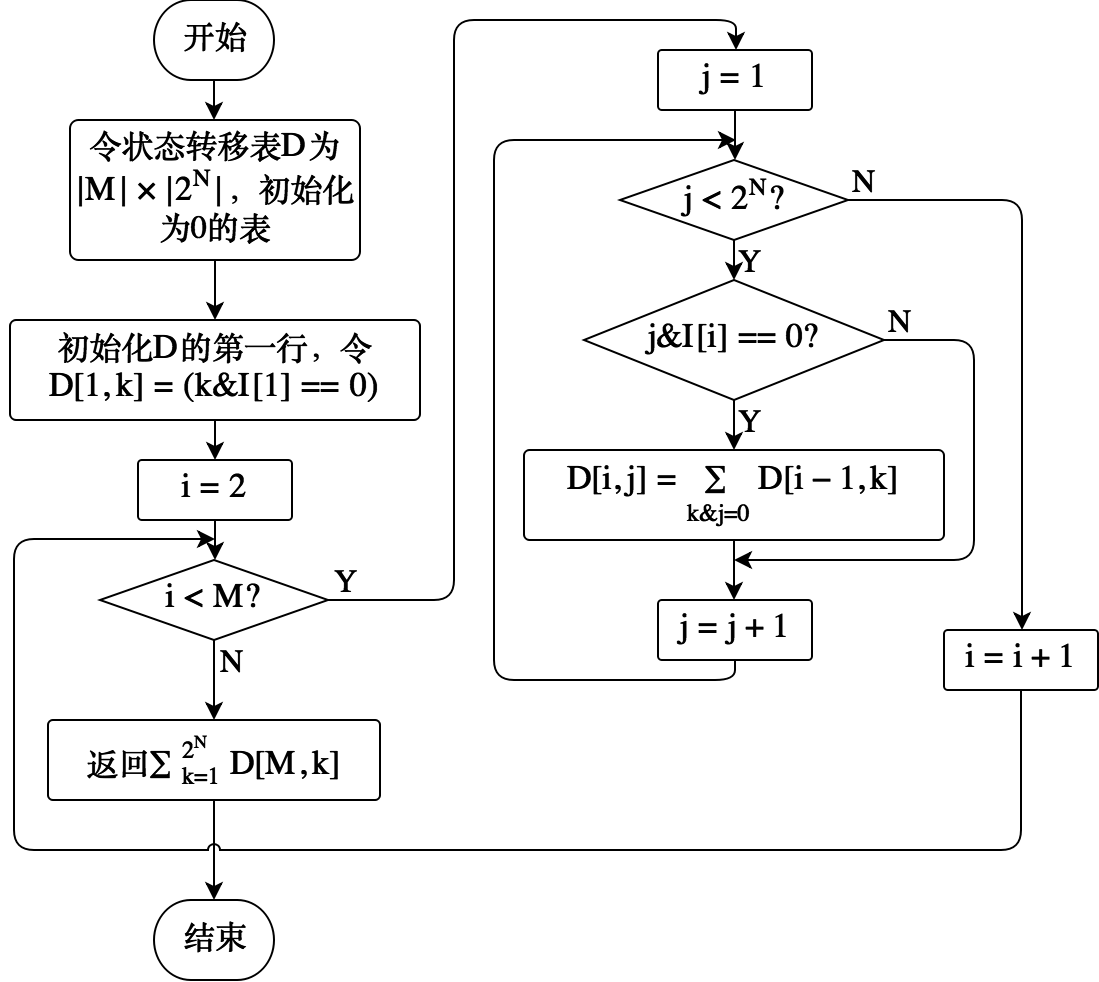
\includegraphics[width=0.6\linewidth]{flowchart7.png}
    \caption{程序流程图}
    \label{fig:flowchart7}
\end{figure}

\section{测试分析}
\label{sec:ce_shi_fen_xi_7}
如\ref{fig:result7}所示,对于POJ提供的测试用例,程序在1MS内全部通过,由此可以说明程序运行正确。

\begin{figure}[ht]
    \centering
    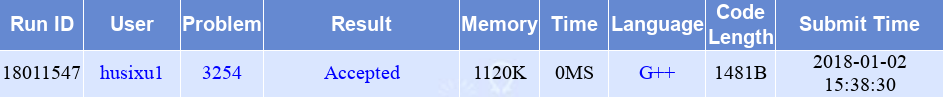
\includegraphics[width=0.9\linewidth]{result7.png}
    \caption{POJ测试结果}
    \label{fig:result7}
\end{figure}

\section{技术总结}
\label{sec:ji_zhu_zong_jie_7}
解决本题的关键在于使用状态压缩,利用一个数的不同二进制位来表示多个实体的二元状态,这样既能够节省空间也能够批量计算节省所需要花费的时间。此外,能够成功的找到状态转移表的两个维度也是解决本题的基础,这一步需要配合状态压缩来完成。

% Chapter Eight %%%%%%%%%%%%%
%%%%%%%%%%%%%%%%%%%%%%%%%%%%%
\chapter{Paid Roads (POJ 3411)}
\label{cha:paid_roads_poj_3411_}

\section{题目描述}
\label{sec:ti_mu_miao_shu_8}
\subsection{Description}
A network of m roads connects $N$ cities (numbered from 1 to $N$). There may be more than one road connecting one city with another. Some of the roads are paid. There are two ways to pay for travel on a paid road $i$ from city $a_i$ to city $b_i$ :
\begin{itemize}
    \item in advance, in a city $c_i$ (which may or may not be the same as $a_i$);
    \item after the travel, in the city $b_i$.
\end{itemize}

The payment is $P_i$ in the first case and $R_i$ in the second case.\par

Write a program to find a minimal-cost route from the city 1 to the city $N$.

\subsection{Input}
The first line of the input contains the values of N and m. Each of the following m lines describes one road by specifying the values of $a_i, b_i, c_i, P_i, R_i (1 \leq i \leq m)$. Adjacent values on the same line are separated by one or more spaces. All values are integers, $1 \leq m, N \leq 10, 0 \leq P_i , R_i \leq 100, P_i \leq R_i (1 \leq i \leq m)$.\par

\subsection{Output}
The first and only line of the file must contain the minimal possible cost of a trip from the city 1 to the city $N$. If the trip is not possible for any reason, the line must contain the word 'impossible'.

\subsection{Sample Input}
\begin{lstlisting}
4 5
1 2 1 10 10
2 3 1 30 50
3 4 3 80 80
2 1 2 10 10
1 3 2 10 50
\end{lstlisting}

\subsection{Sample Output}
\begin{lstlisting}
110
\end{lstlisting}

\section{算法设计}
\label{sec:suan_fa_she_ji_8}
本题是单源最短路径算法的一个扩充,可以使用每个节点带有状态的dijkstra算法实现。但观察题目发现存在$1 \leq m, N \leq 10$这一条件,也就是说城市的数量和路的数量都不超过10,是一个非常小的数据集,因此最终采用了较为简单的深度优先搜索(DFS)来解决本题。\par
使用递归调用自身的方法实现深度优先搜索,在每一层递归时判断当前递归的这一条边所对应的$c_i$是否在已经经过了的那些城市中,若是则使用较低的价格$P_i$,否则使用$R_i$,在搜索时需要注意递归的结束条件,由于总共只有10条边,因此在经过某个城市5次后即可断定已经进入死循环,可以结束当前递归,因此在每层递归中传入一个表$V$来表示每个城市经过的次数,传入$n$表示当前递归的城市,此外到达终点也需要结束当前递归。最终实现的算法如下:
\begin{simpleAlgorithm}{PaidRoads问题求解算法}
    \Procedure{PaidRoads}{$V, n$}
        \If{$n = N$}
            \State \Return 0;
        \EndIf
        \If{$V[n] \geq 5$}
            \State \Return $\infty$;
        \EndIf
        \State $minSum \gets \infty$
        \For{each node $b_i$ adjacent to node $n$} \Comment{与当前节点$n$相邻的每个节点}
            \If{$V[c_i] \neq 0$}
                \State $sum \gets P_i$
            \Else
                \State $sum \gets R_i$
            \EndIf
            \State $V[b_i] \gets V[b_i] + 1$
            \State $p \gets $ \Call{PaidRoads}{$V, b_i$} \Comment{从当前节点到$b_i$的花费}
            \State $V[b_i] \gets V[b_i] - 1$
            \If{$p \neq \infty$}
                \State $sum \gets sum + p$
                \If{$sum < minSum$}
                    \State $minSum \gets sum$;
                \EndIf
            \EndIf
        \EndFor
        \State \Return $minSum$
    \EndProcedure
\end{simpleAlgorithm}

算法对应的流程图如\ref{fig:flowchart8}所示。在每一层递归开始钱,首先判断是否已经到达终点,若是则返回0,否则判断是否是第5次访问当前节点,若是则返回$\infty$表示不能从这一节点找到到达终点的路径。之后对于当前节点的所有邻接节点进行遍历并递归调用自身,来找到从当前节点到终点的最短路径,并返回。若不能找到最短路径则返回$\infty$。此算法的调用者只需传入初始化为0的列表$V$以及节点1即可。

\begin{figure}[ht]
    \centering
    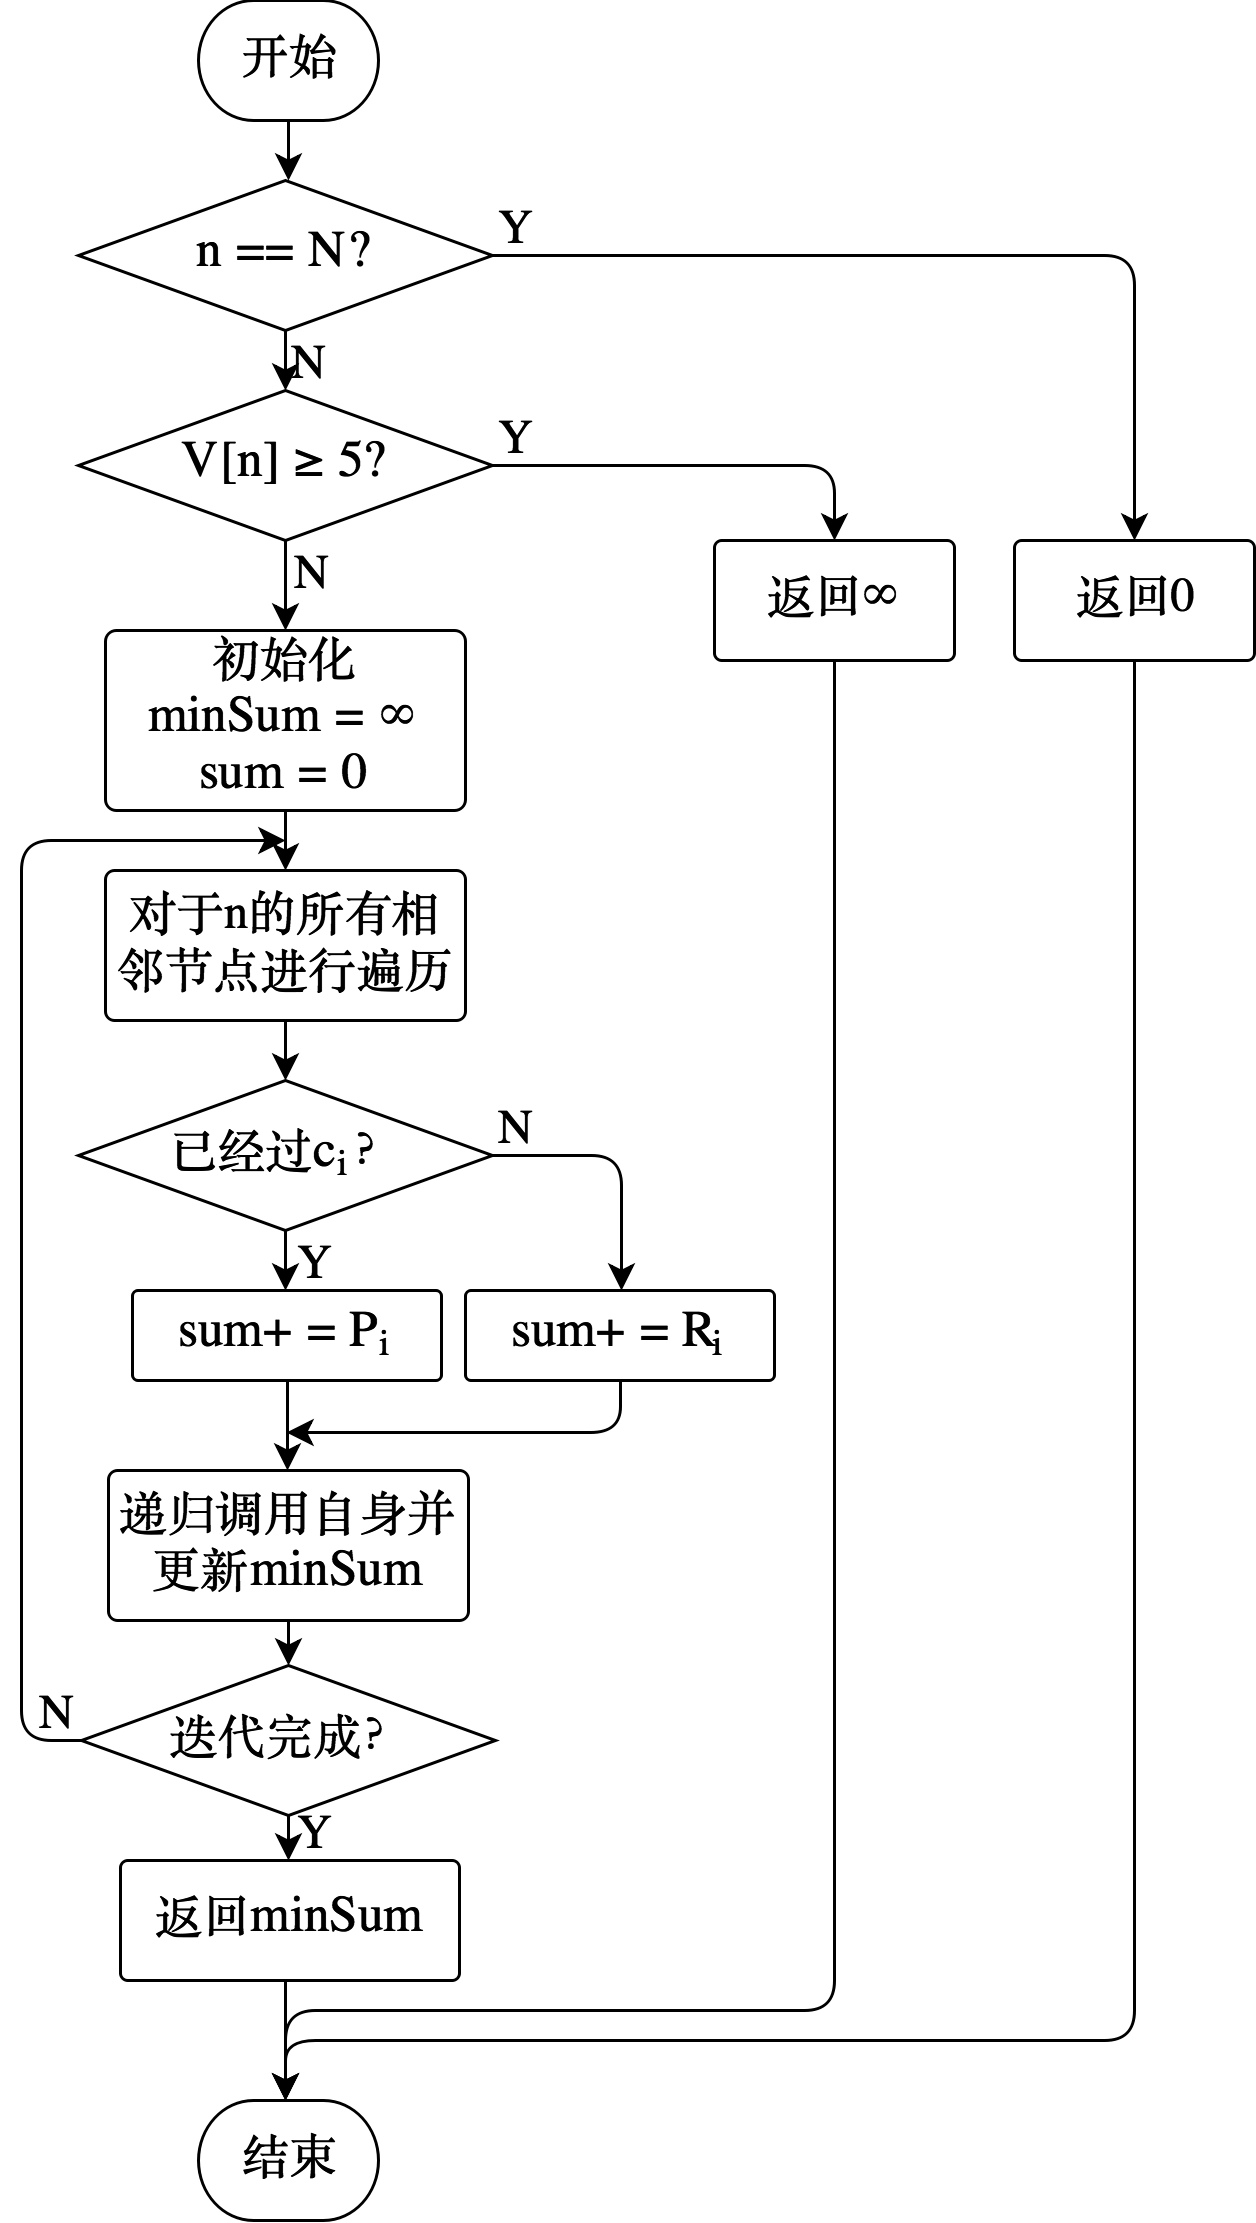
\includegraphics[width=0.4\linewidth]{flowchart8.png}
    \caption{程序流程图}
    \label{fig:flowchart8}
\end{figure}

\section{测试分析}
\label{sec:ce_shi_fen_xi_8}
如\ref{fig:result8}所示,对于POJ提供的测试用例,程序在32MS内全部通过,由此可以说明程序运行正确。

\begin{figure}[ht]
    \centering
    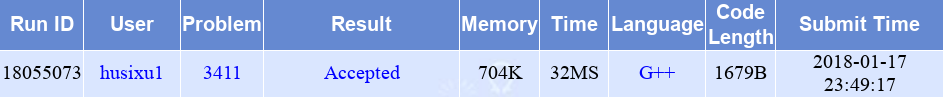
\includegraphics[width=0.9\linewidth]{result8.png}
    \caption{POJ测试结果}
    \label{fig:result8}
\end{figure}

\section{技术总结}
\label{sec:ji_zhu_zong_jie_8}
实现本算法最重要的部分就是找到递归停止的条件,以及每一层递归根据已经经过的路径进行判断,只要能够正确的对于这两个条件进行判断,就能够在较短的时间内对于整个图正确地完成DFS。


% Chapter Eight %%%%%%%%%%%%%
%%%%%%%%%%%%%%%%%%%%%%%%%%%%%
\appendix
\chapter{源代码}
\label{cha:yuan_dai_ma_}

\section{最近点对问题源代码}
\label{cha:zui_jin_dian_dui_wen_ti_yuan_dai_ma_}
\inputCode{../1/main.cpp}

\section{大数乘法源代码}
\label{cha:da_shu_cheng_fa_yuan_dai_ma_}
\inputCode{../2/main.cpp}

\section{最优二分查找树源代码}
\label{cha:zui_you_er_fen_cha_zhao_shu_yuan_dai_ma_}
\inputCode{../3/main.cpp}

\section{Floyd-Warshall最短路径算法源代码}
\label{sec:floyd_warshallzui_duan_lu_jing_suan_fa_yuan_dai_ma_}
\inputCode{../4/main.cpp}

\section{Wooden Sticks(POJ 1065)算法源代码}
\label{sec:wooden_sticks_poj_1065_suan_fa_yuan_dai_ma_}
\inputCode{../5/main.cpp}

\section{Gone Fishing(POJ 1042)算法源代码}
\label{sec:gone_fishing_poj_1042_suan_fa_yuan_dai_ma_}
\inputCode{../6/main.cpp}

\section{Corn Field(POJ 3254)算法源代码}
\label{sec:corn_field_poj_3254_suan_fa_yuan_dai_ma_}
\inputCode{../7/main.cpp}

\section{Paid Roads(POJ 3411)算法源代码}
\label{sec:paid_roads_poj_3411_suan_fa_yuan_dai_ma_}
\inputCode{../8/main.cpp}

\vfill
{\tiny written by 胡思勖 \hfill powered by \XeLaTeX .}
\end{document}
